% =====================================================================
%  COMPARISON ARTIFACT — full adoption of the official SoCS template
%  (mproj.cls + times, per the shipped sample). Same chapter content as
%  dissertation.tex, which remains the canonical document.
%  Build: report/build.sh report/dissertation  (builds both mains)
% =====================================================================
\documentclass{mproj}

\usepackage{graphicx}
\usepackage[T1]{fontenc} % force NFSS/T1 so the PSNFSS Times below applies under XeTeX too
\usepackage{times}   % the shipped template sample loads times over the class's newcent
\usepackage{amsmath,amssymb}
\usepackage{booktabs}
\usepackage{array}
\usepackage[section]{placeins}
\usepackage{enumitem}
\usepackage{caption}
\usepackage[dvipsnames]{xcolor}
\usepackage{tikz}
\usetikzlibrary{positioning,arrows.meta,calc}
\usepackage[numbers,sort&compress]{natbib}
\usepackage[nottoc]{tocbibind} % as in the template sample: puts the bibliography in the ToC
\usepackage[hidelinks]{hyperref} % template renders plain black text; links stay clickable

\setlist{nosep,leftmargin=1.4em}
\captionsetup{font=small,labelfont=bf}

% Float spacing. By default a float page distributes its slack as 1fil above, 2fil between
% floats and 1fil below, which opens huge gaps between a figure and a table sharing a page;
% pin floats to the top, cap the inter-float gap, and let the bottom absorb the remainder.
\setlength{\textfloatsep}{10pt plus 2pt minus 2pt}
\setlength{\intextsep}{10pt plus 2pt minus 2pt}
\setlength{\floatsep}{10pt plus 2pt minus 2pt}
\makeatletter
\setlength{\@fptop}{0pt}
\setlength{\@fpsep}{10pt plus 1fil}
\setlength{\@fpbot}{0pt plus 1fil}
\makeatother
\renewcommand{\topfraction}{0.85}
\renewcommand{\textfraction}{0.1}
\renewcommand{\floatpagefraction}{0.75}

\begin{document}

\title{Predicting the Zero-Shot Transfer of a Promptable Video Tracker}
\author{Kostiantyn Boiar}
\date{\today}
\maketitle

\begin{abstract}
Conservation teams increasingly monitor wildlife with camera traps, which record far more footage than
anyone can watch. Locating each animal in a video and following it from frame to frame is the bottleneck,
and a new generation of promptable trackers promises to remove it: name an animal in ordinary words and the
model finds and follows every one that appears, without ever having been trained on that species. SAM\,3 is
the current example. The difficulty is that this ability is uneven in ways nobody can anticipate --- strong
on one animal or location, poor on the next --- so a team pointing such a model at a new species has no way
of judging beforehand whether to trust its output or fall back on manual annotation.

This dissertation asks whether that judgement can be made in advance. It tests a natural intuition: that a
model should struggle most on the animals and places least like those it has seen before. Were that true,
one could measure how unfamiliar a species or a setting is --- cheaply, without labelling anything and
without running the model at all --- and use the measurement to forecast reliability. Four such measures of
unfamiliarity are tested, and the question is put separately to two distinct abilities: finding the animal
at all, and keeping the identities straight once it has been found.

The answer is that it does not work. On a large camera-trap benchmark of wild animals, no measure of
unfamiliarity predicts performance on species or places the model has not seen. The only property that
predicts anything is how large the animal appears in frame --- a nuisance rather than a discovery --- and a
second attempt based on how difficult the footage looks, such as darkness and visual clutter, collapses into
that same size effect. The finding is not an accident of one dataset or one model: it survives on a second,
independent dataset and on two further trackers of quite different design. Nor is it a failure of method,
since the same test reliably detects the size effect whenever it is present.

The contribution is therefore a carefully bounded negative result, the first for this class of model, and
with it a practical caution: resemblance to familiar training data is no guarantee that such a tracker will
work, and reliability has to be checked rather than assumed.
\end{abstract}

\educationalconsent

\newpage
\section*{Acknowledgements}
I thank my supervisor, Dr Marwa Mahmoud, for guidance throughout this project.

\tableofcontents
\listoffigures
\listoftables

\chapter*{List of Abbreviations}
\addcontentsline{toc}{chapter}{List of Abbreviations}
\begin{tabular}{@{}p{2.7cm}p{11.2cm}@{}}
\texttt{pHOTA}   & Promptable Higher Order Tracking Accuracy --- the benchmark's tracking score \\
\texttt{pDetA}   & Its \emph{detection} half: were the right animals found? (our primary target) \\
\texttt{pAssA}   & Its \emph{association} half: was each identity kept over time? \\
HOTA             & Higher Order Tracking Accuracy, the metric \texttt{pHOTA} derives from \\
IoU              & Intersection over Union, the mask/box overlap measure \\
\addlinespace
GLM              & Generalised Linear Model (here a support-weighted logit-link regression) \\
CI               & Confidence Interval (throughout, a $95\%$ group-cluster-bootstrap interval) \\
MAE              & Mean Absolute Error \\
$\Delta$MAE      & Out-of-sample MAE gain over a mean predictor; positive $=$ better than guessing the mean \\
LSO / LLO        & Leave-Species-Out / Leave-Location-Out cross-validation \\
VIF              & Variance Inflation Factor, a collinearity diagnostic \\
LMG              & Lindeman--Merenda--Gold, the dominance-analysis variance split \\
MMD              & Maximum Mean Discrepancy, a distributional distance \\
\addlinespace
OOD              & Out-Of-Distribution \\
ATC              & Average Thresholded Confidence, an after-running accuracy estimator \\
GT               & Ground Truth \\
IR               & Infrared (night-time camera-trap imagery) \\
RLE              & Run-Length Encoding, the COCO mask format \\
LVIS             & Large Vocabulary Instance Segmentation, the class vocabulary BURST uses \\
\end{tabular}

\chapter{Introduction}
\label{ch:introduction}

\section{Motivation}
Finding an animal in a video and following it over time is a need shared by several fields. Ecologists use it
to survey wild populations from camera-trap footage. Neuroscientists and behavioural biologists use it to
quantify what an animal does frame by frame in the laboratory, where the tracked trajectory is often the
measurement the science rests on, and where a whole tool-chain now exists to recover pose and turn it into
behavioural labels~\cite{deeplabcut,sleap,poser}. The bottleneck is the same in both cases: video is cheap to
record and expensive to annotate.

This dissertation works on the wild side of that divide, where the problem is hardest. Camera traps have
become a standard tool in wildlife monitoring, and a single survey leaves a team with far more footage than
anyone can watch. Somebody still has to work out which animal is in each clip, how many there are, and what
they do. Done by hand this is slow and expensive, and it is the step that limits how much ecology gets done at
all.

Automating it means solving two problems, not one. The first is \emph{finding} the animal in a frame. The
second is \emph{following} it from frame to frame, so the same individual keeps the same identity for as long
as it is visible. Only the second yields the counts and behavioural sequences both communities want: in a
study of social behaviour, losing an identity means losing the very animal whose behaviour was being measured.
It is also the harder of the two.

Neither is easy on real footage. Animals are frequently camouflaged against the very background they live in.
They appear at any distance and from any viewpoint, so one species may fill the frame in one clip and occupy a
handful of pixels in the next. Vegetation cuts them in half. Much footage is recorded at night in infrared,
where colour is gone and contrast is poor. Motion blur is common. A box drawn around the animal is often a
poor description of it, which is why segmentation --- labelling the pixels that belong to the animal --- is
the more useful output. And because a camera trap is fixed, the same cluttered scene repeats in every clip
from that site. That gives a model an easy shortcut: learn the background rather than the
animal~\cite{terra,panaf,xiao}.

For years the standard answer was to train a detector on a fixed list of species and deploy it. It works where
it was trained. It degrades sharply at camera sites and regions it has not seen~\cite{terra,wilds,panaf}. And
adding a species that was not on the list means collecting and labelling more data --- precisely the cost a
team opening a new site is trying to avoid.

Promptable models change that arrangement. The \emph{Segment Anything} line replaced the fixed label set with a
prompt: you indicate what you want and the model segments it, and SAM\,2 extended this to
video~\cite{sam2}. SAM\,3~\cite{sam3} takes the step that matters here, because the prompt can now simply be a
phrase. Give it \texttt{"impala"} and it finds, segments and follows every impala in the clip, having never
been trained on that species. It is the current state of the art for the task, and it was released alongside
SA-FARI, a large camera-trap tracking benchmark of wild animals~\cite{safari}. A team can now point a tracker
at a species it has never seen and get an answer straight away.

That is the appeal. The liability is that the answer is not equally good everywhere. Zero-shot performance
varies sharply from one animal to the next, and from one place to the next. No rule tells a practitioner,
before running the model, whether its output can be trusted for a given animal in a given place. The choice
left is an unattractive one: trust the output blindly, or fall back on the manual annotation the model was
meant to replace.

This dissertation studies that gap. It asks whether such a rule exists --- first for SAM\,3, and then whether
whatever we find is specific to it.

\section{Problem statement and research question}
This dissertation asks whether a promptable tracker's zero-shot accuracy on an unseen (species, place) can be
predicted in advance from properties measurable without running the model or scoring its output, and which
factors govern
that transfer --- separately for finding the animal and following it. We study this concretely on
SAM\,3 as the primary case, measuring novelty against the SA-FARI reference split (Section~\ref{sec:bg-safari}),
and then test whether the answer generalises beyond one dataset and one model --- to two further datasets and,
via a controlled model swap, to two other promptable trackers (Section~\ref{sec:model_swap}).

\section{Hypotheses}
\begin{description}[leftmargin=2.6em,style=nextline]
  \item[H0 (null)] the label-free distances carry no predictive information about
    \texttt{pDetA}/\texttt{pAssA} --- transfer is not distance-driven.
  \item[H1 (detection)] \texttt{pDetA} falls with species novelty (taxonomic + visual distance).
  \item[H2 (association)] \texttt{pAssA} falls with environment difficulty (scene distance,
    day/night/IR, clutter).
\end{description}
Failing to reject H0 is itself an informative result --- and, as Chapter~\ref{ch:results} shows, it is
what we find: neither a novelty distance nor a follow-up intrinsic-difficulty pivot predicts
transfer beyond a trivial animal-size effect. We even read familiarity from SAM\,3's own features, and it too is
null; a fuller representational probe --- of what those features structurally encode --- remains the open
branch for future work.

\section{Contributions}
To our knowledge this is the first study to test, out of sample, whether the zero-shot transfer of a
promptable video tracker can be predicted before the model is run and from label-free distances --- and the
first to split that question into detection (\texttt{pDetA}) and association (\texttt{pAssA}). This distinguishes it
from label-free performance prediction for classifiers, which estimates a single scalar from the model's own
outputs on the target~\cite{aotl,agl,atc}, and from the very recent static-image detector/segmenter
estimators~\cite{pcr,rca}; and from camera-trap shift studies, which measure but do not forecast per-site
reliability~\cite{terra,panaf,jeon}. Concretely we deliver:
\begin{enumerate}[label=(\roman*),leftmargin=2.4em]
  \item a rigorous, out-of-sample negative result --- under a deliberately powerful test (whole-species
    and whole-location hold-out with group-cluster-bootstrap significance), label-free before-running distances
    do \emph{not} predict SAM\,3's transfer;
  \item the detection-versus-association decomposition, tested on two near-orthogonal splits --- a constructed
    species hold-out (novelty) and the official location hold-out (environment);
  \item a hardened account of why it fails: a follow-up intrinsic-difficulty pivot collapses to the
    same animal-size confound, so the only label-free property that predicts detection is object size --- the
    very nuisance the analysis controls for --- and that positive control confirms the test detects signal when
    it exists;
  \item evidence that the null is not an artefact of one dataset or one model: it holds across
    two datasets (SA-FARI and BURST) and, in a controlled model swap on BURST, across two
    architecturally distinct promptable trackers (GLEE and Florence-2\,+\,SAM\,2), so it is task-general rather
    than a quirk of SAM\,3.
\end{enumerate}

\section{Dissertation outline}
Chapter~\ref{ch:background} reviews the related work; Chapter~\ref{ch:methodology} describes the data,
measurement, distance features, and modelling; Chapter~\ref{ch:results} reports the results and
out-of-sample validation; Chapter~\ref{ch:discussion} discusses them; Chapter~\ref{ch:conclusion} concludes.

\chapter{Background and Related Work}
\label{ch:background}

This chapter reviews the work this dissertation builds on. It covers the class of model under study, the
difficulties that make animal detection and tracking hard in the first place, how tracking is scored, the
literature on estimating a model's performance without labels, what is known about distribution shift in
camera-trap vision, the representations that make a distance between species meaningful, and the datasets
involved. It closes by stating the gap that remains.

\section{Promptable and open-vocabulary segmentation and tracking}
\label{sec:bg-promptable}
For most of the last decade, detection and segmentation models were trained against a fixed list of
categories. Such a model cannot be asked about anything outside that list. Extending it to a new category
means collecting labelled examples and training again. In camera-trap work the standard tool of this kind is
MegaDetector~\cite{megadetector}, a detector trained on millions of camera-trap images to localise animals,
people and vehicles, and widely deployed as a first-pass filter over survey footage.

The \emph{Segment Anything} line broke the fixed-list assumption. It replaced the label set with a prompt: a
user indicates what should be segmented, and the model returns a mask for it. SAM\,2~\cite{sam2} carried the
formulation from images to video, propagating a mask across frames from a point or box placed in one of them.

SAM\,3~\cite{sam3} changes what the prompt may be. Instead of a point or a box it accepts a short noun
phrase, and returns every instance matching that phrase, segmented and tracked across the clip. The category
need never have been seen in training. This is a zero-shot, open-vocabulary detect--segment--track
capability, and SAM\,3 is the current state of the art for it.

Other models reach open-vocabulary video understanding by different routes. GLEE~\cite{glee} trains a single
unified model to detect, segment and track objects at scale, driven by a text query. Florence-2~\cite{florence2}
takes a caption-style approach, using one sequence-to-sequence model across a range of vision tasks and
emitting regions in response to a task prompt, though without a confidence score attached to them. These are
the main alternative designs in the same space.

\section{What makes animals hard to detect and track}
\label{sec:bg-challenges}
Wild footage is an unusually hostile input, and the difficulties are worth setting out because they are what
any tracker deployed on it must survive.

The first is that animals are often hard to see at all. Many are camouflaged against the habitat they live
in, and the resulting low contrast between object and background defeats methods that assume a visually
salient foreground. This is a recognised problem in its own right: camouflaged object detection is studied as
a separate task with dedicated benchmarks, precisely because standard detectors underperform on
it~\cite{cod}.

The second is variability of appearance. A camera trap is triggered by whatever passes, so an animal may fill
the frame in one clip and occupy a few dozen pixels in the next. It may face the lens or present only a
flank, and vegetation frequently occludes part of it. A bounding box is a poor description of an animal in
such conditions, which is one reason segmentation --- labelling the pixels belonging to the animal --- is the
more informative output.

The third is image quality. Much wildlife footage is captured at night under infrared illumination, where
colour information is absent and contrast is poor. Infrared and thermal imaging are established wildlife
monitoring modalities with their own detection characteristics, and their properties differ enough from
daylight imagery that observation strategies are designed around them~\cite{thermalwildlife}. Motion blur is
common, since animals are typically moving when they trigger the camera.

The fourth is context. A camera trap is fixed, so the same scene recurs in every clip from that site, and a
model can come to rely on the scene rather than on the animal. This failure mode has a literature of its own,
reviewed in Section~\ref{sec:bg-cameratrap}.

The fifth applies to tracking rather than detection. Keeping an identity attached to the right animal is a
distinct problem from finding it. Animals leave the frame and re-enter it, pass behind vegetation, and in
groups may be near-indistinguishable from one another. Identity errors are treated as a first-class failure
mode in multi-object tracking benchmarks, which annotate visibility explicitly and report identity switches
separately from misses~\cite{motchallenge}. Recovering the identity of a specific individual across sightings
is hard enough in wildlife imagery to constitute its own research area~\cite{animalreid}.

\section{Evaluating multi-object tracking}
\label{sec:bg-hota}
Multi-object tracking is scored by comparing predicted tracks against annotated ones. The difficulty is that
two very different failures --- missing the object, and swapping its identity --- both reduce a single
accuracy figure, and earlier metrics combined them in ways that were hard to interpret.

Higher Order Tracking Accuracy (HOTA)~\cite{hota} was introduced to separate them. At each localisation
threshold $\alpha$ it forms a detection term (\texttt{DetA}: were the right objects found?) and an
association term (\texttt{AssA}: were identities kept consistent over time?), then combines them as a
geometric mean:
\begin{equation}
  \mathrm{HOTA}_\alpha=\sqrt{\mathrm{DetA}_\alpha\cdot\mathrm{AssA}_\alpha},
  \qquad
  \mathrm{pHOTA}=\frac{1}{|\mathcal{A}|}\sum_{\alpha\in\mathcal{A}}\mathrm{HOTA}_\alpha ,
  \label{eq:phota}
\end{equation}
averaged over the threshold set $\mathcal{A}=\{0.05,0.10,\dots,0.95\}$. Because the two terms are formed
separately before being combined, a HOTA score can be read either as a single number or as two.

SA-FARI scores promptable tracking with \texttt{pHOTA}, a promptable variant that decomposes identically into
\texttt{pDetA} and \texttt{pAssA}.

\section{Predicting model performance without labels}
\label{sec:bg-predictable}
A now-mature literature shows that a model's performance under distribution shift can be anticipated without
labelling the target data.

\citet{aotl} observe that out-of-distribution (OOD) accuracy is strongly linearly correlated with
in-distribution accuracy, across many models and many shifts. \citet{agl} show that the agreement between a
pair of models tracks OOD accuracy closely enough to estimate it from unlabelled data alone. A parallel
strand reads the model's own statistics on the unlabelled target. Average thresholded confidence~\cite{atc}
calibrates a confidence threshold on source data and reads off target accuracy as the mass above it, while
\citet{autoeval} regress classifier accuracy directly on a distribution-shift feature --- the Fr\'echet
distance between train and test feature sets.

The idea has only recently reached structured outputs. \citet{pcr} estimate object-detection performance
without ground truth, from the spatial consistency and confidence reliability of pre-NMS boxes. Reverse
classification accuracy~\cite{rca} predicts per-image segmentation quality by training a reverse model
against a labelled reference.

Two properties characterise essentially all of this work. First, the target is an image classifier scored by
a single scalar, or at most a detector or segmenter operating on a static image. None of it concerns identity
maintained over time, and none decomposes the estimate into separate components. Second, every one of these
methods runs the model on the target and inspects what comes out --- its predictions, its confidences, or its
agreement with another model. Each estimates the score of a model that has already been executed.

\section{Distribution shift in camera-trap and wildlife vision}
\label{sec:bg-cameratrap}
That camera-trap models degrade at new locations is well established. \emph{Terra Incognita}~\cite{terra}
showed that recognisers excellent at trained camera sites fail sharply at unseen ones. WILDS~\cite{wilds}
consolidated this, via iWildCam, as a canonical real-world shift. PanAf-FGBG~\cite{panaf} demonstrated that
behaviour-correlated backgrounds causally drive the drop, and proposed a latent-space mitigation.

The claim that scene context, rather than the object, drives such failures has a longer pedigree in general
vision. \citet{xiao} isolate foreground from background on ImageNet, in the ImageNet-9 ``Background
Challenge'', and show that a classifier scores well above chance from the background \emph{alone}. An
adversarially chosen background flips a correctly classified foreground up to $87.5\%$ of the time.
Background is genuine signal, not noise. \citet{elephant} make the parallel point for detectors:
transplanting an object into an unfamiliar scene suppresses its detection, flips its predicted identity as it
moves, and disturbs other detections in the image, exposing a reliance on context and co-occurrence.

\citet{xiao} also report that more accurate and more robust models rely on background \emph{less}, which
suggests the effect is not fixed but a property of how strong the model is.

What this literature shares is its direction of travel. It measures degradation after the fact, or intervenes
on the input to mitigate it. It does not forecast per-site or per-species reliability in advance. It also
studies classifiers and behaviour recognisers rather than promptable trackers, scored by a single accuracy
with no detection/association split.

\section{Representations of species and scenes}
\label{sec:bg-representations}
Measuring how far one species sits from another, or one scene from another, requires a representation in
which such a distance means something.

Vision foundation models turn out to carry that structure. BioCLIP~\cite{bioclip} shows that a model trained
on a large biological image corpus encodes taxonomic structure across the tree of life, its feature space
reflecting the hierarchy that runs from kingdom down to species. Appearance and phylogeny are correlated, so
a representation that separates species visually will tend also to order them taxonomically.

General-purpose encoders offer the same service without biological supervision. DINOv2~\cite{dinov2} learns
visual features self-supervised, and they transfer across domains without fine-tuning. CLIP~\cite{clip}
aligns images with natural-language descriptions, producing a space in which images and text share
coordinates. Both are widely used as off-the-shelf feature extractors.

\section{Datasets}
\label{sec:bg-safari}
Two datasets are central to this work.

\paragraph{SA-FARI.} SA-FARI~\cite{safari} is a large open multi-animal camera-trap tracking dataset,
released alongside SAM\,3. It contains $11{,}609$ densely annotated videos spanning $99$ species, recorded at
$741$ locations across four continents. Every species carries a seven-level biological taxonomy running from
kingdom to species, and every video carries a creation timestamp. Annotations are per-frame masks with
persistent identities, and the benchmark ships an official evaluator, \texttt{VEval}.

Two features set it apart. The taxonomy makes the relationship between two species measurable rather than a
matter of judgement, and the location and timestamp metadata do the same for place and era. The benchmark
also includes abundant \emph{hard negatives}: prompts naming a species that is absent from the clip, which a
correct run should answer with nothing. These make it possible to study false alarms alongside misses.

SA-FARI ships a train/test partition drawn along locations, so the test camera sites are unseen while most
species occur on both sides of it.

\paragraph{BURST.} BURST~\cite{burst} is a video benchmark for object recognition, segmentation and tracking,
built on the TAO~\cite{tao} video corpus. It annotates $482$ categories from the LVIS~\cite{lvis} vocabulary
with per-frame masks and persistent track identities, and a portion of that vocabulary is animal categories.
Its footage comes from internet, driving and film sources rather than camera traps, and it carries neither
location nor timestamp metadata. It is mask-native and considerably more varied in subject matter than
SA-FARI, which makes it a useful independent point of comparison.

\section{Summary and gap}
\label{sec:bg-gap}
Predictable OOD generalisation is established for classifiers scored by a scalar~\cite{aotl,agl,atc,autoeval}
and, very recently, for static detectors and segmenters~\cite{pcr,rca}. Camera-trap vision has thoroughly
documented, but not forecast, location-driven degradation~\cite{terra,wilds,panaf}. Most tellingly, a recent
unified study of camera-trap recognition over time~\cite{jeon} explicitly names ``predicting when zero-shot
models will succeed at a new site'' as an open question, and stops at naming it.

No prior work predicts, \emph{before running the model} and from label-free distances, the zero-shot transfer
of a promptable video tracker. None separates that prediction into detection and association. That is the gap
this dissertation addresses.

\chapter{Data and Methodology}
\label{ch:methodology}

This chapter sets out how the question posed in Chapter~\ref{ch:introduction} was turned into something a
dataset can answer. It begins with the research design, the terms that design depends on, and the rule by
which a predictor counts as validated. It then describes the data and the two splits, how the tracker's
performance is measured, and how the label-free features are computed against a frozen reference. The
remaining sections cover the statistical model and the tests applied to it, the replication on a second
dataset and a second tracker, and the constraints that make the work reproducible.

\section{Research design and evaluation criteria}
\label{sec:meth-design}
This is a predictive-modelling study. On one side is a set of predictors $X$: four distances,
each measuring how far a target species or place sits from a frozen reference, none of them requiring the
tracker to be run or the target to be labelled. On the other is a target $Y$: the tracker's per-cell detection
and association scores. The question is whether $X$ predicts $Y$, and which parts of it do the work, asked
separately for the two halves of the task. Nothing here attempts to make the tracker score higher --- it is the
fixed object of study. Three things need pinning down first: what running it zero-shot means, what the two
scores are, and what would count as having predicted them.

\subsection{What ``zero-shot'' means here}
\label{sec:meth-zeroshot}
A model is run zero-shot on a category when it is asked to find that category without having been trained on
labelled examples of it, and without any change to its weights at the time of asking. The only thing telling it
what to look for is the prompt. A conventional detector, by contrast, is trained on a fixed list and can be
asked about nothing else; a fine-tuned model has had its weights updated on target-domain data; a few-shot
model is handed a small number of labelled examples. A zero-shot model gets the word \texttt{"impala"} and
nothing more.

Three commitments follow and hold throughout. The tracker is the public released checkpoint, and its weights
are never updated --- not fine-tuned, not adapted, not calibrated on any part of this data. The only input
identifying the target is the text prompt. And no labelled example of the target species ever reaches the
tracker: the ground-truth masks are read afterwards, to score what it produced and to crop images when building
the distance features (Section~\ref{sec:meth-features}), never to tell it what to look for. The only thing
fitted anywhere in this study is the small regression mapping distances onto scores. Note that zero-shot is
meant relative to the dataset and to the reference frozen inside it, not as a claim about SAM\,3's undisclosed
pretraining corpus --- a scope limit taken up in Section~\ref{sec:limitations}.

\subsection{What is being predicted: finding and following}
\label{sec:meth-targets}
The evaluator compares what the tracker produced against what a human annotated. Both sides consist of
masklets, a masklet being one object's mask followed through the clip frame by frame, and a predicted mask
counts as matching an annotated one when their intersection over union reaches a threshold $\alpha$. Given that
matching, \texttt{pDetA} (detection accuracy) asks whether the right animals were found, rewarding annotated
animals that were located and penalising both animals missed and masks invented where no animal was.
\texttt{pAssA} (association accuracy) asks whether identities were kept, measuring across the matched
detections how consistently one predicted identity corresponds to one annotated identity over time; it falls
when one animal's track is split among several predicted identities, when two identities are swapped, and when
two animals are merged into a single track.

Both lie in $[0,1]$, higher is better, and both are averaged over $\alpha\in\{0.05,\dots,0.95\}$, so neither
depends on one arbitrary choice of how much overlap is close enough (Equation~\ref{eq:phota}). The mask-based
variants are used throughout, SA-FARI being mask-annotated, and neither metric is reimplemented: the official
\texttt{VEval} evaluator is run as supplied and its output read.

The two are not symmetric, and the asymmetry matters. Association is conditional on detection, since an
identity can only be assessed for an animal that was found in the first place. A second consequence is worth
flagging at the outset. Where a clip holds a single animal there is only one identity to keep, so
\texttt{pAssA} is then largely determined by \texttt{pDetA} and carries little variance of its own. How often
that happens is a property of the data rather than of the design, and Chapter~\ref{ch:discussion} reports it;
where it dominates, association is reported as the weak target it is rather than as an independently powered
test. The external replication of Section~\ref{sec:meth-replication} was chosen partly because it does not have
this problem.

\subsection{Definition of success and the decision rule}
\label{sec:meth-success}
The intended deliverable is a validated, out-of-sample predictor of \texttt{pDetA}/\texttt{pAssA} from
label-free distances, with confidence intervals that respect the group structure
(Section~\ref{sec:meth-inference}). A distance is taken to predict transfer only if it clears both bars:
\begin{enumerate}[label=(\roman*),leftmargin=2.4em]
  \item its coefficient's group-cluster-bootstrap 95\% confidence interval (CI) excludes zero; and
  \item the grouped cross-validated model beats a mean-predictor baseline by a margin that is significant under
    a paired group-bootstrap.
\end{enumerate}
The bars are not redundant. Criterion~(i) says a relationship is visible in the data the model was fitted on;
it does not say that relationship holds for a species or place never seen, which is the entire practical claim.
Criterion~(ii) is that test, and its baseline is deliberately humble --- predicting each held-out cell with the
training mean, which is what a practitioner with no predictor would effectively assume. A feature clearing (i)
but not (ii) has been fitted, not validated.

H1 (detection $\leftarrow$ species novelty) and H2 (association $\leftarrow$ environment difficulty) are
supported only when their respective distances meet this bar on the split that isolates them. If neither does
under tests built deliberately to be powerful, the conclusion is H0 --- distance explains little variance ---
which is a substantive result rather than a failure to find one, and motivates the representational-probing
direction of Chapter~\ref{ch:discussion}.


\section{Data, splits, and the analysis unit}
\label{sec:meth-data}
SA-FARI~\cite{safari} is the primary dataset, and everything in this section describes it. The independent
replication runs on a second dataset, BURST, which Section~\ref{sec:meth-replication} covers separately.

Each test is a probe: one video paired with one text prompt. The prompt names a species, which resolves its
taxonomy, and the video supplies the location and the timestamp. Probes are then aggregated into cells, a cell
being one (species, location, time) group. Each cell carries support counts ($n_\text{frames}$,
$n_\text{masklets}$, $n_\text{videos}$), used for weighting and as covariates. The cell is the unit of
analysis throughout: it is what carries a score, and what the regression is fitted on.

Hard negatives --- prompts naming a species that is absent --- are kept, because they carry the false-positive
side of detection. There is one exception. The large pooled inference pass uses a stratified per-species cap to
remain feasible, and under that cap hard negatives are set aside from inference and analysed separately
instead (Section~\ref{sec:meth-fp}).

\paragraph{Two complementary splits.}
SA-FARI's shipped split separates locations but not species (Section~\ref{sec:bg-safari}). Species-distance is
therefore $\approx\!0$ for nearly every cell, so that split cannot test species novelty on its own. Because the
tracker is frozen (Section~\ref{sec:meth-zeroshot}), the shipped split plays no training role and serves only
to define our reference distribution, which leaves us free to repartition the same videos. Inference is run
once --- scoring is per-video and split-agnostic --- and two splits are overlaid on the result:
\begin{description}[leftmargin=1.6em,style=nextline]
  \item[Split A --- species hold-out (primary).] Species from both official splits are pooled and held out one
    at a time, so a held-out species' distance is measured to the nearest remaining species. Species-distance
    varies while the environment stays familiar, which isolates H1.
  \item[Split B --- location hold-out (secondary).] The official split, whose unseen locations isolate H2, and
    whose comparability with the published benchmark carries the initial score-sanity check.
\end{description}
Split A is a constructed hold-out rather than a shipped one. That is legitimate precisely because the model is
frozen, and it is reported as constructed throughout.

Split B yields $1{,}447$ scored cells, spanning $113$ taxonomy-bearing categories and $92$ unseen test
locations. Of those cells $346$ are positive, meaning the queried species is present so that \texttt{pDetA} and
\texttt{pAssA} are defined; the remaining $1{,}101$ are hard negatives, drawn from $1{,}486$ hard-negative
probes. Split A pools the species present in both official splits into $1{,}025$ scored cells.

\section{Measuring transfer}
\label{sec:meth-measure}
Figure~\ref{fig:pipeline} sets out the pipeline as a whole. This section describes its upper path: how the
frozen tracker is run and scored into the target $Y$. Sections~\ref{sec:meth-features}
and~\ref{sec:meth-model} describe the lower path and the modelling.

\begin{figure}[htbp]
\centering
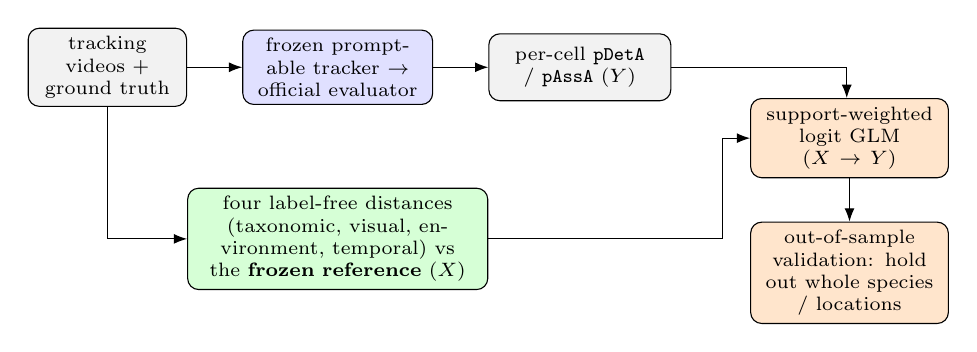
\begin{tikzpicture}[>=Latex, node distance=0.9cm, every node/.style={font=\scriptsize},
  b/.style={draw, rounded corners, align=center, inner sep=3pt, minimum height=0.85cm},
  d/.style={b, fill=black!5}, m/.style={b, fill=blue!12},
  f/.style={b, fill=green!16}, g/.style={b, fill=orange!20}]
  % top row: the frozen measurement path X-fixed, producing the target Y
  \node[d, text width=1.8cm] (vid) {tracking videos + ground truth};
  \node[m, text width=2.2cm, right=0.7cm of vid] (sam) {frozen promptable tracker $\to$ official evaluator};
  \node[d, text width=2.1cm, right=0.7cm of sam] (y) {per-cell \texttt{pDetA} / \texttt{pAssA} ($Y$)};
  % bottom row: the label-free predictor path
  \node[f, text width=3.6cm, below=1.05cm of sam] (dist)
    {four label-free distances (taxonomic, visual, environment, temporal) vs the \textbf{frozen reference} ($X$)};
  % modelling column on the right
  \node[g, text width=2.3cm, right=1.0cm of y, yshift=-0.9cm] (glm) {support-weighted logit GLM \;($X\!\to\!Y$)};
  \node[g, text width=2.3cm, below=0.55cm of glm] (cv)
    {out-of-sample validation: hold out whole species / locations};
  \draw[->] (vid) -- (sam);   \draw[->] (sam) -- (y);
  \draw[->] (vid.south) |- (dist.west);
  \draw[->] (y.east)    -| ([xshift=-1pt]glm.north);
  \draw[->] (dist.east) -- ([xshift=-10pt]dist.east -| glm.west) |- (glm.west);
  \draw[->] (glm) -- (cv);
\end{tikzpicture}
\caption[The measurement-and-modelling pipeline]{The measurement-and-modelling pipeline, identical for every
dataset and tracker. \emph{Top:} the frozen tracker is scored by the official evaluator into per-cell
detection/association scores (the target $Y$). \emph{Bottom:} four label-free distances are computed against a
frozen reference (the predictors $X$). A support-weighted logit GLM relates $X$ to $Y$, validated out of sample
by holding out whole species and locations. Only the GLM is fitted; the tracker is never trained.}
\label{fig:pipeline}
\end{figure}

The primary case is SAM\,3 on SA-FARI, and the rest of this section gives its concrete choices and numbers.
The replication and the model swap (Sections~\ref{sec:meth-replication}--\ref{sec:meth-swap}) later re-run the
same pipeline on other datasets and trackers.

SAM\,3~\cite{sam3} is run frozen over the probe videos and scored with the official \texttt{VEval} evaluator,
which yields a per-cell \texttt{pDetA}, \texttt{pAssA} and \texttt{pHOTA}~\cite{hota} together with its
support. Species-specific prompts are the primary condition, and a generic ``animal'' prompt is run as a
robustness check. One inference pass over the union of the Split~A and Split~B probes serves both experiments.
Predictions are keyed per (video, species), so that the several prompts issued against a single video cannot
collide, and the harness can resume video by video.

The frame-level scores are aggregated two ways, and the two are kept distinct. The micro score is the
dataset-level \texttt{VEval} figure, reported only to confirm that we reproduce the published SA-FARI operating
point of $\approx\!0.65$ mask-\texttt{pHOTA}. The macro score is the support-weighted mean over positive cells,
and it is the modelling target: the model is fitted cell by cell, so the cell is what must carry a score. Being
a positives-only per-cell average, the macro mean sits lower, at $\approx\!0.53$. Unless a figure is explicitly
identified as the micro score, every measurement number quoted in this dissertation is the macro value.

\paragraph{Validity of the frozen protocol.} Because the tracker is frozen throughout
(Section~\ref{sec:meth-zeroshot}), reusing that single inference pass across both splits is sound rather than a
leak: a cell's score cannot depend on which reference partition is later overlaid to compute its distances.

Freezing also settles the benchmark's status. SA-FARI is a held-out, zero-shot benchmark for the released
SAM\,3. The SAM\,3 report~\cite{sam3} does not list SA-FARI among its training sources, and the SA-FARI
paper~\cite{safari} reports the released checkpoint zero-shot, alongside separately fine-tuned rows whose gain
we deliberately forgo. Non-membership can therefore be verified at the dataset level. It cannot be verified
frame by frame, because SAM\,3's full pretraining corpus is undisclosed. That is why every distance is measured
against the SA-FARI reference rather than against whatever SAM\,3 actually saw, and why the familiarity proxy
of Section~\ref{sec:meth-familiarity} is included as a hedge.

\section{Label-free distance features}
\label{sec:meth-features}
The features defined here fall into three groups. Four are distances, one for each axis along which a target
can be unfamiliar: taxonomic, visual, environment and temporal. These four are the hypothesis variables, with
H1 resting on the first two and H2 on the third. The second group holds a single nuisance covariate, animal
size. The third holds the familiarity proxy.

For each split, the reference (``seen'') species, locations and taxonomy are frozen once, and every distance is
then computed against that reference alone. This is the leakage firewall: no information about a probe can
enter a feature. A unit test verifies it, swapping the reference and checking that the distances move as
expected. We assert the axis that is genuinely disjoint --- location for Split~B, the held-out species for
Split~A --- and report any residual species overlap rather than asserting it away.

Because the distances are computed against that reference, they require no measurement of the tracker's
performance on the target: no \texttt{pDetA}, no \texttt{pAssA}, no annotation of how well SAM\,3 did. That is
the sense in which they are label-free, and it is the sense the research question needs, since it makes them
available before the model is run.

One qualification belongs here rather than in a footnote. As implemented on an annotated benchmark, the visual,
environment and size features read the dataset's ground-truth masks to separate animal from scene. That is a
convenience of working on SA-FARI, not a requirement of the method: in deployment the same species prototype
would be built from the handful of exemplar images a practitioner already has for a named species. It does
bound the claim, and Section~\ref{sec:limitations} returns to it.
\subsection{Taxonomic distance}
This distance measures how far apart two species sit on the tree of life.

Every species carries a seven-level path from kingdom down to species. Write that path $\pi(s)$, and let
$\mathrm{shared}(a,b)$ count the levels on which two paths agree, starting from the top. Two species are then
as far apart as the number of levels they do not share. A cell's distance is the smallest such value over the
reference set $\mathcal{R}$:
\begin{equation}
  \tau(a,b)=L-\mathrm{shared}(a,b)\quad (L=7),
  \qquad
  d_{\mathrm{tax}}(s)=\min_{s'\in\mathcal{R},\;s'\neq s}\tau\big(\pi(s),\pi(s')\big).
  \label{eq:taxdist}
\end{equation}

So a species sharing a genus with its nearest reference neighbour scores $1$, a shared family $2$, and a shared
order $3$. A species sharing no level at all would score $7$. The exclusion $s'\neq s$ is the leave-species-out
rule, which keeps the measure non-trivial for species present on both sides of a split. Species whose taxonomy
is incomplete are left undefined rather than imputed.
\subsection{Visual distance}
This distance measures how different one species looks from another.

Each animal is cropped to its ground-truth mask, with the background zeroed, and embedded with
DINOv2~\cite{dinov2}. A species is then summarised by a single prototype: the mean of its embeddings,
renormalised to unit length. The distance from an embedding $v$ to the nearest prototype other than its own is
one minus the largest cosine similarity,
\begin{equation}
  p_j=\frac{\bar v_j}{\lVert \bar v_j\rVert_2},
  \qquad
  d_{\mathrm{vis}}(v)=1-\max_{j\neq e}\, v^{\!\top}p_j ,
  \label{eq:protodist}
\end{equation}
where $e$ indexes the query's own species, excluded again under the leave-species-out rule. A
CLIP~\cite{clip} encoder replaces DINOv2 as a robustness check. The masks come from the annotations
(Figure~\ref{fig:features}b).
\subsection{Environment distance}
This distance measures how different one scene looks from another.

The animal is erased from the frame, its pixels replaced by the mean colour of what remains, and the result is
embedded exactly as above (Figure~\ref{fig:features}c). Here prototypes are formed per location rather than per
species, and $d_{\mathrm{env}}$ is Equation~\ref{eq:protodist} applied to the nearest other location.

Three interpretable covariates come from the same frames. Infrared footage is greyscale, so a pixel's spread
across colour channels, $\max_c f_c-\min_c f_c$, collapses towards zero; a frame counts as achromatic when that
spread averages below $12$. The low-light fraction is the share of a location's frames that are achromatic, and
the night/IR flag is that fraction exceeding one half. Clutter is the mean variance of a Laplacian over the
greyscale background, which measures local edge and texture density rather than colour.

\begin{figure}[htbp]
\centering
\begin{minipage}[b]{0.32\textwidth}\centering
  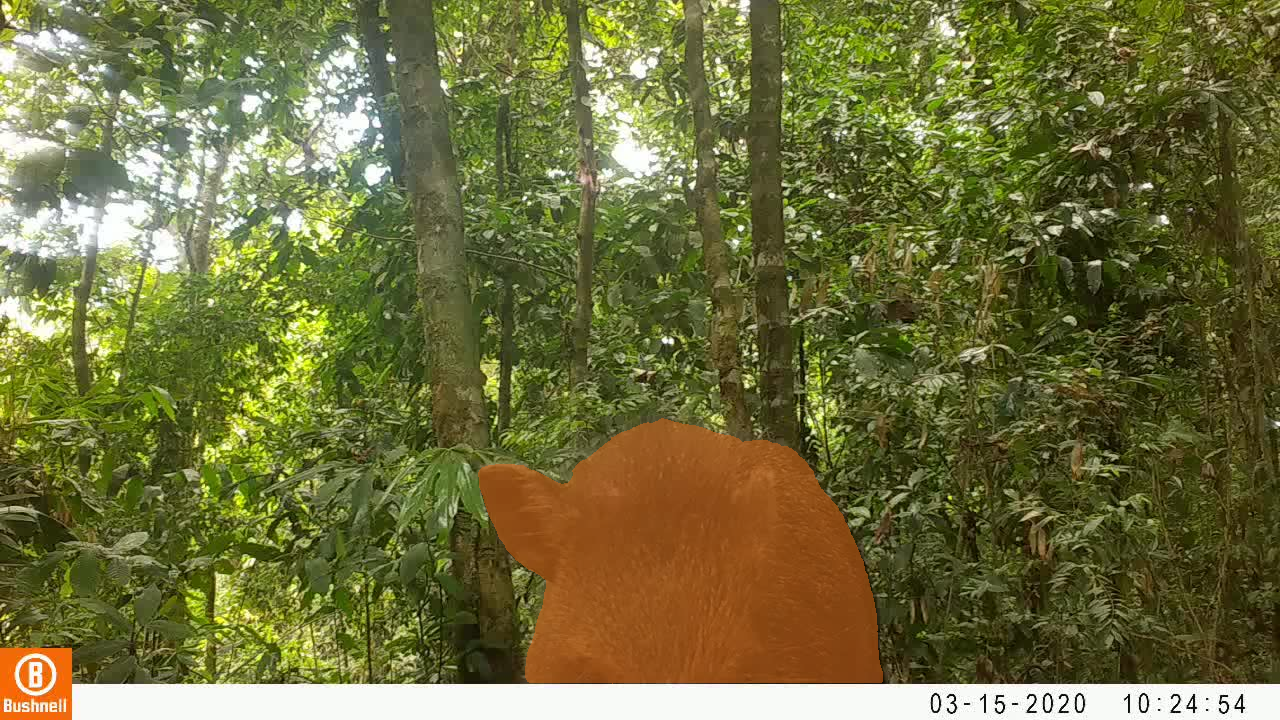
\includegraphics[width=\linewidth]{figures/feat_overlay.png}\\[2pt]{\footnotesize (a) frame $+$ ground-truth mask}
\end{minipage}\hfill
\begin{minipage}[b]{0.32\textwidth}\centering
  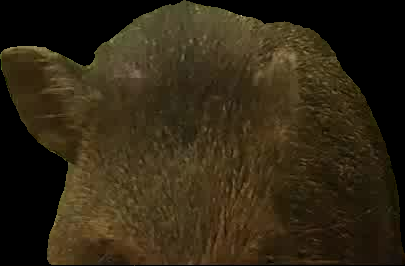
\includegraphics[width=\linewidth]{figures/feat_animal.png}\\[2pt]{\footnotesize (b) visual: mask-cropped animal}
\end{minipage}\hfill
\begin{minipage}[b]{0.32\textwidth}\centering
  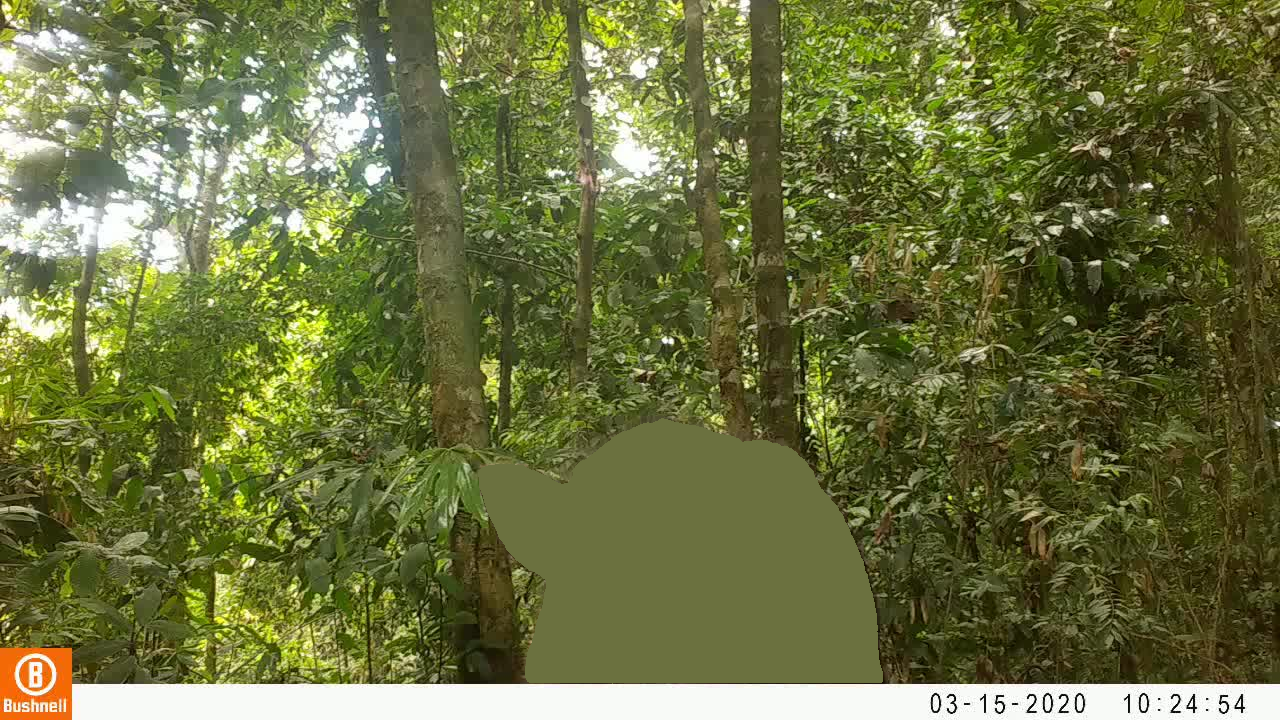
\includegraphics[width=\linewidth]{figures/feat_background.png}\\[2pt]{\footnotesize (c) environment: animal erased}
\end{minipage}
\caption[The image-based distances in action]{The two image-based distances on a camera-trap frame (a collared
peccary). \textbf{(a)} ground-truth mask (orange); \textbf{(b)} the mask-cropped animal the visual
distance fingerprints; \textbf{(c)} the animal mean-inpainted, which the environment distance
fingerprints. None of these features runs SAM\,3.}
\label{fig:features}
\end{figure}

\subsection{Temporal gap}
\label{sec:meth-temporal}
This distance measures how far apart in time two recordings were made.

Years come from the per-video creation-datetime metadata. For a cell recorded in year $y$, the gap is the
smallest absolute difference to any reference year in $\mathcal{Y}$:
\begin{equation}
  d_{\mathrm{temp}}=\min_{r\in\mathcal{Y}}\,|y-r| .
  \label{eq:tempgap}
\end{equation}

The feature depends on timestamps being both present and varied across cells. How far the available metadata
actually supports it is reported in Chapter~\ref{ch:results}.
\subsection{Animal size (confound control)}
This covariate measures how large the animal appears in frame.

Let $a$ be a species' mean ground-truth mask area in pixels, averaged over sampled masklets. The covariate is
$\ln(1+a)$. Larger animals are easier to segment, so this is what separates genuine visual novelty from mere
conspicuousness. Section~\ref{sec:meth-model} describes how it is used to test whether an apparent novelty
effect is really a size effect.
\subsection{SAM\,3 familiarity proxy}
\label{sec:meth-familiarity}
This feature measures how familiar a species looks to SAM\,3 itself.

Every distance above is measured against the SA-FARI reference rather than against what SAM\,3 actually saw
(Section~\ref{sec:meth-measure}). The proxy hedges that gap by reading familiarity from the model. The same
mask-cropped animals used for the visual distance are pushed through SAM\,3's image encoder, and the
patch-token features are mean-pooled into a $1024$-dimensional vector. Each species is then scored three ways:
by silhouette, comparing own-cluster compactness against the nearest other species; by nearest prototype, which
is Equation~\ref{eq:protodist} recomputed with SAM\,3's encoder in place of DINOv2; and by Mahalanobis
typicality against the reference feature Gaussian.

The proxy stays before-running and label-free. It is a property of the images, not a function of SAM\,3's
tracking output, so it is not circular. Each of the three metrics is validated at the same leave-species-out
bar, Bonferroni-corrected across them, and size-controlled. The decisive question is whether any of them adds
out-of-sample gain over the visual distance and size together (Section~\ref{sec:familiarity}).

\section{Statistical modelling and hypothesis testing}
\label{sec:meth-model}
Section~\ref{sec:meth-measure} produced the target $Y$, and Section~\ref{sec:meth-features} the predictors $X$.
This section relates the two, and puts the decision rule of Section~\ref{sec:meth-success} into practice.

Its order follows that rule. The first subsection fits the model, the second derives the confidence intervals
that criterion~(i) tests, and the third the out-of-sample comparison that criterion~(ii) tests. The fourth
divides explained variance between predictors that overlap. The fifth and sixth put two further questions that
the four distances do not reach: whether intrinsic difficulty predicts better than novelty, and whether novelty
predicts false alarms rather than misses. The last checks that the outcome does not hinge on any single design
choice.

\subsection{Per-target regression}
\label{sec:meth-per-target}
Detection and association are modelled separately, because their decomposition is the intellectual core of the
project. Section~\ref{sec:meth-targets} gives the qualification. Association may carry little variance
independent of detection, in which case it is reported as the weaker target rather than as an independently
powered test.

Each target is bounded in $[0,1]$. Each is therefore modelled with a support-weighted logit-link, or
fractional-logit, regression:
\begin{equation}
  \operatorname{logit}\mathbb{E}[y]=x^{\!\top}\beta,
  \qquad\text{fit with variance weights } w=n_{\mathrm{frames}},
  \label{eq:glm}
\end{equation}
where $y$ is the cell's score and $x$ the standardised design. That design carries the four distances, the
scene covariates, and a $\log(n_\text{frames})$ term. The last of these is what keeps ``rare'' from being
mistaken for ``far''.

\subsection{Group-aware confidence intervals}
\label{sec:meth-inference}
A naive model interval would be far too narrow here, for two reasons. Support-weighting by frame count inflates
the effective sample size. And a distance is constant within a species or a location, so hundreds of cells
represent only tens of independent groups, which is pseudo-replication. We therefore resample whole species and
whole locations, refit on each resample, and take percentile intervals. Every coefficient interval reported in
this dissertation is that group-cluster-bootstrap interval.

\subsection{Out-of-sample validation and the significance test}
\label{sec:meth-cv}
Validation holds out whole groups: leave-species-out on Split~A, leave-location-out on Split~B. The model is
fitted without a group, then predicts it. Criterion~(ii) compares the resulting error against the
mean-predictor baseline, and a paired group-bootstrap resampling whole held-out groups tests that comparison.
It returns both a confidence interval and a one-sided $p$-value on the gain.

\paragraph{Distinguishing absence of signal from absence of power.}
A null is only informative if the test could have detected an effect had one been present, so the design
carries a positive control. The animal-size covariate is put through the identical procedure --- the same
clustered interval, the same whole-group hold-out --- and the estimation and cross-validation machinery is
unit-tested to recover planted effects on synthetic data. If the procedure clears the bar for size while
staying flat for the distances, a flat result is evidence of absence of signal rather than absence of power.
Chapter~\ref{ch:results} reports whether it does.

\subsection{Variance attribution and confound control}
\label{sec:meth-variance}
Four univariate fits would not show how much each factor explains, because the distances overlap one another.
Variance is therefore attributed by dominance analysis, which divides shared explanatory power between
correlated predictors, with a VIF check for collinearity. Raw correlations are reported alongside as a
model-free cross-check. Where a distance does reach significance, the model is refitted with the animal-size
covariate, to test whether the effect is size rather than novelty.

\subsection{The intrinsic-difficulty pivot and the nested decomposition}
The novelty distances are not the only label-free properties available. A complementary question, taken up
after the novelty tests were complete, is whether transfer is governed by the intrinsic difficulty of the
target imagery rather than by its novelty. The scene properties already measured for the environment axis ---
the low-light fraction, the clutter score and the night/IR flag --- are promoted from nuisance covariates to
predictors of interest, and tested against the same out-of-sample bar.

Difficulty and size are easily confused, so they are separated by a nested sequence of models: support only,
size only, difficulty without size, and difficulty plus size. Comparing their out-of-sample gains exposes any
apparent difficulty effect that is really size (Table~\ref{tab:difficulty}). Each scene property's cell-level
correlation is also reported beside its location-level value, because aggregating inflates correlations. That
is the ecological-correlation fallacy.

\subsection{Detection precision: false positives on hard negatives}
\label{sec:meth-fp}
The \texttt{pDetA} model conditions on the animal being present, so it measures recall given presence rather
than hallucination. Hard negatives supply the other side. There the queried species is absent, so a correct run
returns no masklet at all.

The predictions are read directly, and any returned masklet scoring above a threshold is flagged as a false
positive. Each species' taxonomic and visual distance is attached, and the test asks whether the hallucination
rate rises with novelty. It is run at the species level rather than the cell level, to avoid pseudo-replication.

\subsection{Design-robustness checks}
\label{sec:meth-robustness}
To test whether the outcome depends on any single design choice, the whole hold-out procedure is re-run with
one component of the pipeline swapped at a time. The visual encoder changes from DINOv2 to CLIP. The crop
changes from the mask-cropped animal to a whole-frame box that keeps the background. The prompt changes from
species-specific to a generic ``animal''. And the visual-distance functional changes from a nearest-prototype
cosine to a distributional Fr\'echet or MMD distance between the target and reference embedding sets, after
AutoEval~\cite{autoeval}. Each variant is fitted and validated at the identical whole-group bar, with
significance judged after a Bonferroni correction over the variant family (Table~\ref{tab:robustness}).

\section{Independent replication on an external dataset}
\label{sec:meth-replication}
Every SA-FARI result reuses one frozen inference pass on one dataset. The two splits are therefore
near-orthogonal, but not statistically independent. To test whether the outcome is a property of the transfer
problem rather than of SA-FARI, the whole pipeline is re-run on a second dataset. Nothing changes but the data:
the same frozen SAM\,3, the same official scorer, the same distances, and the same leave-species-out
cross-validation and paired group bootstrap.

This is cheap because the pipeline is bound to an annotation schema rather than to a loader. An offline adapter
converts the new dataset into the SA-Co JSON that the loader and evaluator already read, so nothing downstream
changes.

\paragraph{BURST.} The replication runs on the animal subset of the BURST validation split
(Section~\ref{sec:bg-burst}): $41$ species across $132$ video\,$\times$\,class cells, scored by mask-HOTA on
the native masks. Animal categories are selected by a WordNet filter~\cite{wordnet}, taking the hyponyms of
\texttt{animal.n.01}, and mapped to the seven-level taxonomy wherever it resolves. It resolves in full for $25$
of the $41$ species, and the rest are left undefined. BURST supplies neither of the metadata axes SA-FARI does,
so the cell key is the per-video sequence and leave-species-out is the only valid grouping. Both
\texttt{pDetA} and \texttt{pAssA} are tested here, at the same bar as SA-FARI and with the same animal-size
positive control (Section~\ref{sec:meth-cv}).

\subsection{The controlled model swap}
\label{sec:meth-swap}
The replication varies the data and holds the tracker fixed. The swap does the reverse. Everything else stays
constant --- the same cells, the same ground truth, the same four distances, the same GLM under
leave-species-out cross-validation --- and SAM\,3 is replaced by another open-vocabulary, text-promptable
tracker. Only \texttt{pDetA} changes, because the distances are functions of the data and its ground truth
rather than of the tracker. That is what isolates the tracker as the sole varying factor, and it is also why
this is a swap rather than a replication.

Two challengers of deliberately different architecture are used. GLEE~\cite{glee} is a single unified
detect--segment--track model. Florence-2~\cite{florence2} paired with SAM\,2~\cite{sam2} is a caption-style box
generator, carrying no confidence score, followed by a mask-propagating tracker.

Two safeguards keep the swap fair. The first is a measurement gate. A challenger's per-cell \texttt{pDetA} must
show real spread across cells before any regression is fitted on it. A regression on scores floored at zero has
no variance to explain and would report a spurious null, so a challenger scoring $\approx 0$ on a dataset is
dropped there rather than modelled.

The second concerns scoring fairness. Open-vocabulary detectors calibrate their confidence to their own
training domain, so a near-zero score may reflect the evaluator's confidence gate rather than a real detection
failure. Every such score is therefore re-checked under a box-based metric, and again under a threshold-free
average-precision metric with no gate at all. This gate is also what decides which dataset can host a fair
swap, and it is why the swap runs on BURST rather than SA-FARI; Chapter~\ref{ch:results} gives the measurements
behind that choice. Each challenger configuration is fixed in advance from the model's own defaults, run once,
and reported as-is (Section~\ref{sec:model_swap}).

\section{Reproducibility and implementation}
\label{sec:meth-repro}
The constraints that protect validity are stated where they apply: the frozen tracker
(Section~\ref{sec:meth-zeroshot}), the official evaluator (Section~\ref{sec:meth-targets}), the frozen
reference (Section~\ref{sec:meth-features}), and the retained hard negatives (Section~\ref{sec:meth-data}).
What remains is how they are enforced.

Each is a configuration toggle rather than a branch in the code, so an ablation changes a config file and
nothing else. The pipeline is covered by hermetic tests, among them the leakage check of
Section~\ref{sec:meth-features} and the recovery of planted effects on synthetic data. Split definitions,
random seeds and reference sets are all persisted. Every number reported in this dissertation comes from that
pipeline, and both experiments reproduce end to end.

All inference is single-GPU and inference-only, since no weights are ever updated.

\chapter{Results and Evaluation}
\label{ch:results}

% Tables under tables/ are generated by `python -m src.analysis.report` from outputs/ and committed.
% The \IfFileExists guards let the dissertation build whether or not they have been generated yet.

This chapter reports what the measurements show. It opens by checking that the frozen tracker reproduces the
published benchmark. It then works through the model in the order the decision rule of
Section~\ref{sec:meth-success} demands: the fitted coefficients, how much variance the distances explain
together with the intrinsic-difficulty pivot, and the out-of-sample test that settles the research question.
Further sections cover the species hold-out, false positives on hard negatives, the robustness variants and
the familiarity proxy. The last three take the analysis to a second dataset, draw the cross-dataset synthesis,
and substitute two other trackers. Supporting tables numbered B.* are collected in
Appendix~\ref{app:supplementary}.

\section{Measurement}
\label{sec:measurement}
Before any modelling, the measurement itself has to be sound. Zero-shot SAM\,3 on the SA-FARI test split
reproduces the published benchmark: the dataset-level (micro) \texttt{VEval} score is $\approx\!0.65$
mask-\texttt{pHOTA}, matching the operating point reported with the dataset.

Table~\ref{tab:gate1} reports a different and lower quantity. It gives the three mask metrics --- detection,
association, and their combination --- as support-weighted means over the $346$ positive cells, which is the
form the model is fitted on. Detection, the primary target, sits at $0.527$, and combined \texttt{pHOTA} at
$0.533$. The gap from $0.65$ is not a discrepancy. The micro figure pools every frame in the dataset into a
single score, whereas this one averages within each cell first and counts positive cells only
(Section~\ref{sec:meth-measure}).
\IfFileExists{tables/gate1_measurement.tex}{% generated by src/analysis/report.py --- do not edit by hand
\begin{table}[htbp]\centering
  \caption{Zero-shot SAM\,3 on the SA-FARI test split --- support-weighted mean over 346 scored cells (of 1447).}
  \label{tab:gate1}
  \begin{tabular}{lr}
    \toprule
    Metric (mask) & Value \\
    \midrule
    pDetA & 0.527 \\
    pAssA & 0.546 \\
    pHOTA & 0.533 \\
    \bottomrule
  \end{tabular}
\end{table}
}{}

\section{Fitted coefficients}
\label{sec:coefficients}
This section reports the first of the two criteria a distance must clear (Section~\ref{sec:meth-success}): does
its coefficient's confidence interval exclude zero? Table~\ref{tab:coefficients} answers that for the location
split, Split~B, over the same $346$ positive cells as Table~\ref{tab:gate1}. The species hold-out is reported
separately in Section~\ref{sec:species-holdout}.

Each row of the table is one factor, and the two columns give its coefficient and confidence interval for
detection and for association. Three features of its construction should be noted.

The coefficients are standardised. Each is the change in the logit of the score for a one-standard-deviation
rise in that factor. Magnitudes can therefore be compared down a column, even though the raw factors are in
quite different units: tree steps, cosine gaps, a binary flag. A negative coefficient means the score falls
as the factor rises, which is the direction H1 and H2 predict.

The intervals are not the model's own. A distance is constant within a species or a location, so the $346$
cells behave like only a few tens of independent groups. These intervals resample whole species and whole
locations instead (Section~\ref{sec:meth-inference}). They are wide deliberately, and that width is the real
uncertainty rather than a defect of the data.

Only three of the four distances appear. Temporal gap is absent because it carries no variance to estimate
from and the model drops it (Section~\ref{sec:meth-temporal}). The last two rows are a scene covariate and the
support control rather than distances.

On this reading, no factor satisfies criterion~(i). Every interval spans zero, for detection and
association alike. Criterion~(i) already fails, before the out-of-sample test of Section~\ref{sec:headline} is
reached.

Two further details are relevant. First, the point estimates for taxonomic and visual distance are negative
here, nominally the direction H1 predicts. The intervals are, however, far too wide for that sign to carry
information, and on the species hold-out, where species novelty actually varies, both coefficients are
positive (Section~\ref{sec:species-holdout}), the opposite of what H1 predicts.

Second, taxonomic distance carries by far the widest interval, $[-3.87,+0.09]$ for detection. That is a
property of this split rather than a finding about taxonomy. The official split shares species across train and
test, so taxonomic distance is $\approx\!0$ for almost every cell here, and the coefficient is estimated from
almost no variation. It is measured imprecisely rather than measured and refuted, and is counted as neither.
The constructed species hold-out is designed to test species novelty properly.
\IfFileExists{tables/coefficients.tex}{% generated by src/analysis/report.py --- do not edit by hand
\begin{table}[t]\centering
  \caption{Standardised logit-GLM coefficients (95\% CI) for detection (pDetA) and association (pAssA).}
  \label{tab:coefficients}
  \begin{tabular}{lcc}
    \toprule
    Factor & pDetA coef.\ [CI] & pAssA coef.\ [CI] \\
    \midrule
    Taxonomic distance & -0.362 [-0.41, -0.32] & -0.368 [-0.41, -0.32] \\
    Temporal gap & -0.000 [-0.00, -0.00] & -0.000 [-0.00, -0.00] \\
    Visual distance & -0.144 [-0.17, -0.12] & -0.122 [-0.14, -0.10] \\
    Environment distance & 0.042 [0.02, 0.06] & 0.013 [-0.01, 0.03] \\
    Clutter & -0.066 [-0.09, -0.04] & -0.087 [-0.11, -0.06] \\
    Night / IR & -0.405 [-0.45, -0.36] & -0.462 [-0.51, -0.41] \\
    log(support) & -0.216 [-0.24, -0.20] & -0.224 [-0.24, -0.20] \\
    \bottomrule
  \end{tabular}
\end{table}
}{}

\section{How much the distances explain, and the difficulty pivot}
\label{sec:variance-difficulty}
The first question is how much of the variation in detection the four distances account for. They account
for almost none of it. A dominance analysis puts the four together at only $\approx 3\%$ of the variation, and no single
distance stands out (Table~\ref{tab:variance}). The method is LMG/Shapley, which splits shared explanatory
power fairly between correlated predictors rather than double-counting it.

One possible explanation is that the distances are so correlated with one another that a real effect cancels out
between them. The VIF column rules that out. The variance inflation factor measures how entangled each
predictor is with the others, and a value near $1$ means essentially independent. Every VIF here is
$\approx 1$, so the $3\%$ is the total explanatory contribution rather than a signal masked by collinearity.


The only distance with an apparent predictive relationship was visual distance, and that relationship is
attributable to animal size. Visually distinctive species tend to be larger, and larger animals are easier to
detect. The apparent novelty effect is therefore confounded with size.

A complementary question follows: whether the intrinsic difficulty of the scene, rather than the novelty of
the animal, predicts detection. Three label-free scene properties are tested against the same criteria: low
light, visual clutter, and a night/IR flag (Table~\ref{tab:difficulty}, Appendix~\ref{app:supplementary}).
Each is measured directly from the frames, with no SAM\,3 run and no target label.

Combined with animal size, these difficulty signals improve on the baseline by $+0.017$ and $+0.020$ on the
two hold-outs. Separating the contributions shows that the entire gain comes from size. Size \emph{on its
own} accounts for it. Low light \emph{on its own} does not improve on the baseline, and adds almost nothing
once size is accounted for.

The apparent night/IR effect is inflated by being measured at the wrong level. Per location, its correlation
with detection looks moderate, at $r=-0.377$. That is an averaging artefact. Measured at the level of the
individual cell, where the model actually operates, it shrinks to $-0.13$, and clutter's is $0.00$. The
intrinsic-difficulty hypothesis is therefore \textbf{also null}: the only label-free property that predicts
detection is animal size.


\section{The primary out-of-sample test: predicting unseen species and locations}
\label{sec:headline}
This is the primary test. The model is fitted on a subset of species and locations, then used to predict
detection for held-out species and locations excluded from fitting. Its error is compared against the
simplest baseline: predicting the mean score in every case.

Table~\ref{tab:cv} reports that comparison. Each row is one combination of hold-out scheme and target, so the
four rows cover leave-species-out and leave-location-out for both detection and association, all within the
same $346$ positive cells. The MAE column is the model's mean absolute error, and Baseline is the mean
predictor's. $\Delta$ is the gain of one over the other, so a positive value indicates lower error than the
mean predictor. The interval comes from the paired group-bootstrap, and the $p$-value is one-sided
(Section~\ref{sec:meth-cv}).

The result is a \textbf{null}. Every gain falls between $+0.004$ and $+0.007$, every interval spans zero, and
no $p$-value drops below $0.13$. On both hold-out schemes, and for both targets, the distance model does not
improve on the mean predictor.

Figure~\ref{fig:predvsactual} presents this graphically. Each point is one held-out cell, with its true
detection score on the horizontal axis and the model's out-of-sample prediction on the vertical. A model that
predicted well would place its points along the dashed diagonal. A model that ignored its inputs and returned
the average every time would place them along the horizontal line. The points follow the horizontal line:
the prediction varies negligibly with the true score.

The null is credible because the procedure demonstrably has power. Run unchanged on the same cells, it
\emph{does} recover a real effect. Animal size improves on the baseline out of sample at the identical
criteria, significantly on both schemes ($\Delta\mathrm{MAE}=+0.015$ leave-species-out, $+0.017$
leave-location-out; Table~\ref{tab:difficulty}). A procedure that detects the size effect while returning no
gain for the distances indicates that the distances carry \emph{no} predictive signal: the null result
reflects an absence of signal, and the size result confirms the power to detect one.
\IfFileExists{tables/cv_validation.tex}{% generated by src/analysis/report.py --- do not edit by hand
\begin{table}[htbp]\centering
  \caption[Out-of-sample validation, location split]{Out-of-sample error vs a mean predictor on the \textbf{location split} (Split~B; the $346$ positive
  cells). Each row is one cross-validation grouping scheme --- leave-species-out or leave-location-out ---
  applied within these same cells; $\Delta$ is the MAE gain over baseline, with a paired-bootstrap 95\% CI and
  one-sided $p$. No scheme's gain is significant.}
  \label{tab:cv}
  \begin{tabular}{llrrrcr}
    \toprule
    CV scheme & Target & $n$ & MAE & Baseline & $\Delta$~[95\% CI] & $p$ \\
    \midrule
    location & pAssA & 346 & 0.289 & 0.295 & +0.007~[-0.005,\,+0.018] & 0.13 \\
    location & pDetA & 346 & 0.293 & 0.298 & +0.004~[-0.007,\,+0.015] & 0.23 \\
    species & pAssA & 346 & 0.289 & 0.295 & +0.006~[-0.006,\,+0.017] & 0.16 \\
    species & pDetA & 346 & 0.293 & 0.298 & +0.004~[-0.006,\,+0.015] & 0.24 \\
    \bottomrule
  \end{tabular}
\end{table}
}{}
\begin{figure}[htbp]
\centering
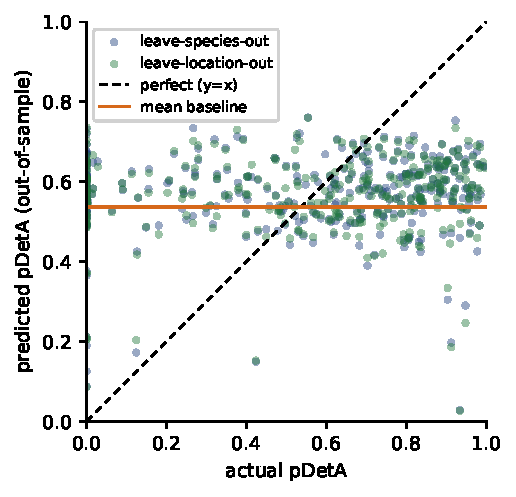
\includegraphics[width=0.44\textwidth]{figures/res_pred_vs_actual.pdf}
\caption[Out-of-sample predicted vs actual]{Out-of-sample detection predictions against the truth, for held-out
species (navy) and held-out locations (green); each point is one cell. Perfect prediction would lie on the
dashed diagonal, and predicting the mean regardless of input lies on the orange horizontal. The points follow
the orange line, so the distances carry no predictive power.}
\label{fig:predvsactual}
\end{figure}

\section{Species hold-out (H1): novelty and the size confound}
\label{sec:species-holdout}
The primary novelty test is a leave-species-out analysis over the pooled train and test species: $99$
species and $1{,}025$ scored cells. Three tables report it, each the Split~A counterpart of one already seen
for Split~B. Table~\ref{tab:gate1_species} (Appendix~\ref{app:supplementary}) gives the measurement, and
confirms the tracker scores in the same range on the pooled set as on the test split alone.
Table~\ref{tab:coefficients_species}, in this chapter, gives the fitted coefficients, and
Table~\ref{tab:cv_species}, also in the appendix, the out-of-sample test.

Out-of-sample prediction again fails. Every gain in Table~\ref{tab:cv_species} is zero or negative, so the
distance model is no better than the mean predictor, and on the species scheme slightly worse.

Table~\ref{tab:coefficients_species} is where this split differs from Split~B. One coefficient does have an interval excluding zero: visual distance, at $+0.37$ for detection. Its sign,
though, is \emph{positive}. Taken at face value, this indicates that more-novel species are detected better,
which is the reverse of what H1 predicts.

It is a \textbf{confound} rather than a reversal. Visually distinctive species tend to be larger
(visual~$\leftrightarrow$~$\log$-area $r=0.22$), and larger animals score higher
($\log$-area~$\leftrightarrow$~\texttt{pDetA} $r=0.30$, the strongest raw correlate of the score). Adding an
animal-size covariate shrinks the visual coefficient from $+0.37$ to $+0.22$, and its interval now spans zero,
while size itself becomes the significant driver. The apparent visual-novelty effect is therefore a size
effect. Taxonomic novelty shows no relationship ($r\approx0.00$).

Figure~\ref{fig:size} shows the same relationship on the location split, where its cell-level correlation is
$r=+0.31$. Each point is one cell, with animal size on the horizontal axis and its detection score on the
vertical. Novelty does not predict transfer; animal size does, weakly.
\begin{figure}[htbp]
\centering
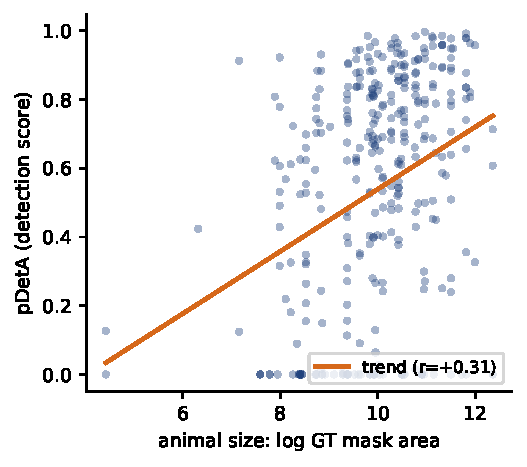
\includegraphics[width=0.44\textwidth]{figures/res_size_confound.pdf}
\caption[The size confound]{The one label-free property that predicts detection: animal size. Per-cell
detection score against log ground-truth mask area, on the location split ($346$ cells), with the fitted trend
at $r=+0.31$. This is the confound behind the apparent visual-distance effect.}
\label{fig:size}
\end{figure}


\IfFileExists{tables/coefficients_species.tex}{% generated by src/analysis/report.py --- do not edit by hand
\begin{table}[htbp]\centering
  \caption{Standardised logit-GLM coefficients with \emph{group-cluster-bootstrap} 95\% CIs (resampling whole species / locations, so the interval respects pseudo-replication and the support weighting), for detection (pDetA) and association (pAssA).}
  \label{tab:coefficients_species}
  \begin{tabular}{lcc}
    \toprule
    Factor & pDetA coef.\ [CI] & pAssA coef.\ [CI] \\
    \midrule
    Taxonomic distance & 0.202 [-0.09, 0.43] & 0.209 [-0.06, 0.42] \\
    Visual distance & 0.369 [0.11, 0.67] & 0.271 [0.04, 0.54] \\
    Environment distance & 0.043 [-0.15, 0.17] & 0.023 [-0.15, 0.13] \\
    Clutter & -0.284 [-0.52, 0.02] & -0.230 [-0.46, 0.06] \\
    Night / IR & -0.286 [-0.77, 0.22] & -0.439 [-0.92, 0.06] \\
    log(support) & -0.020 [-0.14, 0.16] & 0.051 [-0.06, 0.23] \\
    \bottomrule
  \end{tabular}
\end{table}
}{}

\section{False positives / hallucination}
\label{sec:fp}
Everything so far has concerned misses: whether the tracker finds the animals that are there. The detection
score conditions on the animal being present, so it measures recall and is uninformative about hallucination.
The opposite failure (reporting an animal that is not there) is measured on the $1{,}486$ hard negatives, the
queries naming a species absent from the clip. A correct run returns nothing. SAM\,3 nonetheless returns a
masklet in approximately $9.8\%$ of cases.

Table~\ref{tab:fp} asks whether that rate is predictable from the same label-free distances. Each row is one
species-level test, giving the statistic, its $95\%$ confidence interval, and the verdict. The first four rows
are correlations between a species' hallucination rate and one property. The last row is the out-of-sample
test, where the statistic is an MAE gain over a mean predictor rather than a correlation.

This is the closest the study comes to a validated before-running signal. Taxonomic novelty shows no
relationship ($r\approx+0.06$, not significant). Visual distinctiveness does: the more distinctive a species
looks, the \emph{less} the model hallucinates it ($r\approx-0.33$). The relationship remains under an
animal-size control, strengthening to a partial $-0.37$, and size on its own is not significant. Unlike every
earlier effect, this one is not attributable to animal size.

It remains a correlate rather than a predictor. Predicting a held-out species' hallucination rate from visual
distance improves on a mean predictor by only $+0.008$ MAE and does not reach out-of-sample significance
($p=0.053$). Even the strongest signal in the study fails the criterion. Its direction is also the opposite of
the hypothesis: greater distinctiveness is associated with fewer false positives, rather than greater novelty
with worse performance.

\IfFileExists{tables/false_positives.tex}{% generated by src/analysis/report.py --- do not edit by hand
\begin{table}[htbp]\centering
  \caption{False positives on the 1486 hard negatives (113 species): the overall hallucination rate is 9.8\%. More visually distinctive species hallucinate \emph{less} --- a real, size-independent correlate --- but it does not validate out of sample (leave-species-out $p=0.053$), so it is a correlate, not a predictor.}
  \label{tab:fp}
  \begin{tabular}{lccc}
    \toprule
    Test (species-level) & statistic & 95\% CI & verdict \\
    \midrule
    FP rate vs taxonomic distance & $+0.06$ & $[-0.17,\,+0.23]$ & n.s. \\
    FP rate vs \textbf{visual distance} & $-0.33$ & $[-0.43,\,-0.23]$ & significant \\
    \quad visual, size-controlled (partial) & $-0.37$ & $[-0.47,\,-0.28]$ & significant \\
    FP rate vs animal size & $+0.13$ & $[-0.06,\,+0.31]$ & n.s. \\
    leave-species-out OOS gain & $+0.008$ & $[-0.002,\,+0.017]$ & $p=0.053$ \\
    \bottomrule
  \end{tabular}
\end{table}
}{}

\section{Ablations and robustness}
\label{sec:robustness}
The null of Section~\ref{sec:headline} rests on one particular model, built from one particular set of design
choices. This section asks whether either could be responsible for it. The first subsection varies which
factors enter the model. The second holds the factors fixed and varies how they are computed.

\subsection{Factor ablation}
Table~\ref{tab:ablation} (Appendix~\ref{app:supplementary}) refits detection with one change to the design
per row. The pseudo-$R^2$ column is McFadden's, a measure of in-sample fit. The last two columns give the
out-of-sample MAE gain over a mean predictor under the two hold-out schemes, leave-species-out and leave-location-out, each with its $p$-value.

Removing any single distance changes either quantity only marginally, so no single distance carries signal
that the others obscure. Dropping temporal gap changes nothing at all, which is expected: it has no variance and the
model already discards it (Section~\ref{sec:meth-temporal}). Removing the support covariate leaves the model
slightly worse than the baseline ($-0.002$ and $-0.003$), so the null is not that control suppressing a real
effect.

One row does change substantially. Adding the animal-size covariate more than doubles the fit, from $0.055$
to $0.119$, and lifts the out-of-sample gain to significance on both schemes, at $+0.018$ ($p=0.02$) and
$+0.020$ ($p=0.00$) for the full model with the distances included. This is consistent with the variance
partition (Table~\ref{tab:variance}), in which the distances together explain almost nothing.

\subsection{Design robustness}
Table~\ref{tab:robustness} (Appendix~\ref{app:supplementary}) keeps the factor set fixed and swaps a single
design choice per row. Each entry is the out-of-sample gain with its confidence interval and $p$-value, under both hold-out schemes, judged after a
Bonferroni correction over the five variants.

Three swaps test the distances themselves. They change the encoder from DINOv2 to CLIP, take a whole-frame
embedding that keeps the background instead of a mask crop, and replace the nearest-prototype distance with a
distributional Fr\'echet or MMD distance. All leave the gain indistinguishable from the baseline. Every
$\Delta\mathrm{MAE}$ is at most $0.007$, every $p$-value at least $0.10$, and every interval spans zero.

The generic ``animal'' prompt is included for completeness, and produces a different outcome. Prompting
non-specifically collapses per-species detection to a near-constant, mostly-zero target: mean
\texttt{pDetA}$\approx0.14$, with $73\%$ of cells exactly zero. Fitting a target that degenerate, the model
does not merely fail to improve on the mean predictor but falls far below it ($\Delta\mathrm{MAE}\approx-0.35$).

Across every variant the label-free distances fail identically. The null is a property of the transfer
problem, not of one modelling choice.

\section{SAM\,3 familiarity proxy}
\label{sec:familiarity}
Every distance so far has measured novelty against the SA-FARI reference. One objection follows: SA-FARI is
not SAM\,3's training set, and the actual pretraining data is undisclosed, so the distances may fail only
because novelty is measured from the wrong anchor.

The familiarity proxy (Section~\ref{sec:meth-familiarity}) tests that objection by reading familiarity from
SAM\,3 itself, from how separable each species is in its own vision-encoder feature space.
Table~\ref{tab:familiarity} (Appendix~\ref{app:supplementary}) reports the three separability metrics over
the $346$ positive cells. The first two
columns give each metric's out-of-sample gain and $p$-value, on SA-FARI and on BURST. The next two give its
correlation with the DINOv2 visual distance and with animal size, which together show what the metric is really
measuring. The last column is the verdict against a Bonferroni threshold of $\alpha=0.017$ for three metrics.

The result is a further null. None of the three satisfies the criterion on the leave-species-out novelty
test. The strongest, silhouette, reaches only $p=0.034$ for a gain of $+0.012$, and nearest-prototype and
Mahalanobis are further from the threshold, at $p=0.068$ and $0.085$. The null replicates on BURST, where the same three give $p=0.020$,
$0.136$ and $0.148$.

The $r_\text{vis}$ column explains why. All three correlate with the DINOv2 visual distance they re-encode, at
$0.63$ to $0.85$. They largely restate a feature already shown to be null, and in direct comparison none adds
out-of-sample gain over the visual distance plus size. One row differs: silhouette, unlike the
visual distance, is \emph{not} a size artefact ($r_\text{size}=-0.16$). It isolates the size-independent half of
visual distinctness, and still fails to predict transfer.

The metrics do reach significance under leave-location-out ($p\le0.01$), but that is not a novelty test. A
familiarity value is constant within a species, with zero within-species variance. On the location split the
held-out locations' species also appear in training, so a species-constant feature is never tested on an unseen
species at all.

Nor is the null a power failure. On these same $346$ cells the animal-size control does validate out of
sample (Table~\ref{tab:ablation}), so a test returning no gain here reflects an absence of signal rather than
insufficient sensitivity. Reading familiarity from SAM\,3's own representations therefore does not recover
before-running prediction. It restates the same size-entangled visual distinctness that was already null, and
it closes the objection that SAM\,3's true training set is unknown.

\section{Independent replication on a second dataset}
\label{sec:burst}
Both SA-FARI experiments overlay different splits on one frozen inference pass, so they are near-orthogonal
rather than independent (Section~\ref{sec:meth-replication}). BURST~\cite{burst} supplies the independent test:
$132$ cells across $41$ species, mask-native, in a quite different regime of internet, driving and film video
rather than camera traps.

Two preconditions hold there. Zero-shot SAM\,3 is non-degenerate, at \texttt{pHOTA} $0.635$
(Table~\ref{tab:gate1_burst}, Appendix~\ref{app:supplementary}), so there is real variance to model. And the
association target is genuine rather than near-degenerate as it is on SA-FARI: \texttt{pDetA} and
\texttt{pAssA} correlate at $0.76$, and none of the $71$ multi-object cells has them exactly equal. Both components are therefore testable.

Table~\ref{tab:replication_burst} (Appendix~\ref{app:supplementary}) reports the outcome under
leave-species-out cross-validation. Each row is one
predictor, with its out-of-sample MAE gain, confidence interval and $p$-value. The last row is the animal-size
control rather than a distance.

The distances are again null. Combined, they improve out-of-sample error by only $+0.002$ ($p=0.374$), and
individually visual ($+0.003$), taxonomic ($-0.006$) and environment ($-0.001$) are all null. So are the
association specifications. The result survives dropping the $19$ single-cell species, and survives a size
control.

The only near-signal is the same artefact identified above. Visual distance correlates with detection at
$+0.17$ per cell, and at $+0.37$ between species, the same aggregation inflation seen for night/IR in
Section~\ref{sec:variance-difficulty}. Both are \emph{positive}, meaning more-novel animals are detected
better, which is the opposite of the novelty hypothesis. The correlation is also not robust to a size control
(partial $+0.08$, $p=0.35$).

This is a second convergent null rather than positive proof. No before-running quantity reaches significance
here, not even the animal-size control that does validate on SA-FARI. Without a positive control that
reaches significance, the test cannot establish that it would have detected a small species-level effect. What BURST establishes is that no
moderate-or-large before-running distance signal exists in an independent mask-native regime with a genuine
association target. A small species-constant effect cannot be excluded.

\section{Cross-dataset synthesis}
\label{sec:cross_dataset}
Table~\ref{tab:cross_dataset} collects every feature tested, its result on each dataset, and the verdict. The
two dataset columns are not in the same metric, and each header says which it is. BURST entries are
out-of-sample $\Delta$MAE with a $p$-value. SA-FARI entries are standardised GLM coefficients with
confidence intervals, except the rows marked $\dagger$, which are $\Delta$MAE like BURST; the temporal and
hallucination rows report the quantities stated in place. A feature predicts transfer only if it is positive
\emph{and} significant.

The pattern is consistent. No before-running label-free distance, alone or combined, predicts detection or
association transfer out of sample on either dataset, and every gain over a mean predictor sits within
bootstrap noise of zero.

The only near-signal is visual distance, and its direction is the reverse of that predicted: more-novel
animals are detected better, not worse. It does not remain significant under an animal-size control wherever
it is examined.

One row does clear the bar, and it is the confound rather than a hypothesis variable. Animal size validates out
of sample on SA-FARI, modestly. That row doubles as the positive control: the same test that returns no gain
for every distance does detect size, so the null is an absence of signal rather than an absence of power.

The contribution is that null, with its bounds stated and quantified. It is consistent across a camera-trap
dataset and an internet-video one. The clustered intervals cap the visual and environment coefficients at
moderate size, and a planted-effect analysis (Table~\ref{tab:mde}, Appendix~\ref{app:supplementary}) shows
the out-of-sample test reaches $80\%$ power only for standardised effects of $1.5$ (location scheme) to
$1.75$ (species scheme), a gain of $\Delta\mathrm{MAE}\approx+0.02$. Criterion~(ii) therefore certifies the
absence of usable predictive value; effects far smaller than that threshold, including any of the observed
coefficient magnitudes, are bounded by the intervals rather than by the out-of-sample test.
\IfFileExists{tables/cross_dataset_comparison.tex}{% Cross-dataset feature comparison --- hand-maintained; 
\begin{table}[htbp]\centering
  \caption[Cross-dataset synthesis]{Cross-dataset synthesis: every feature tested, per dataset. BURST entries are out-of-sample
  $\Delta$MAE\,($p$); SA-FARI entries are GLM coefficients [95\% CI], except the $\dagger$ rows, which are
  $\Delta$MAE\,($p$) from the species hold-out; the temporal and hallucination rows report the quantities stated in place. Only animal size satisfies the criteria, and only on SA-FARI.}
  \label{tab:cross_dataset}
  \footnotesize
  \setlength{\tabcolsep}{5pt}
  \begin{tabular}{>{\raggedright\arraybackslash}p{3.0cm}ll>{\raggedright\arraybackslash}p{2.8cm}}
    \toprule
    Feature & SA-FARI (coef.\ [CI]) & BURST ($\Delta$MAE, $p$) & Verdict \\
    \midrule
    \multicolumn{4}{l}{\emph{Before-running label-free distances (the research question)}} \\
    Combined distances$^\dagger$ & $-0.004$ ($0.74$)          & $+0.002$ ($0.37$) & null on both \\
    Visual alone                 & $-0.14$ [$-0.50$,\,$0.14$] & $+0.003$ ($0.26$) & null; wrong direction \\
    Taxonomic alone              & $-0.36$ [$-3.87$,\,$0.09$] & $-0.006$ ($0.95$) & null on both \\
    Environment alone            & $+0.04$ [$-0.19$,\,$0.24$] & $-0.001$ ($0.75$) & null on both \\
    Temporal gap                 & $32/1447$, all $=0$        & no timestamps     & untested \\
    \midrule
    \multicolumn{4}{l}{\emph{Confound control}} \\
    Animal size ($\log$-area)$^\dagger$ & $+0.015$ ($0.01$) & $+0.005$ ($0.14$) & \textbf{validates} (SA-FARI) \\
    \midrule
    \multicolumn{4}{l}{\emph{Detection precision (hard negatives)}} \\
    Hallucination vs visual & $r{=}-0.33$; $+0.008$ ($0.053$) & --- & marginal correlate \\
    \bottomrule
  \end{tabular}
\end{table}
}{}

\section{Cross-model replication}
\label{sec:model_swap}
Both datasets above vary the data while holding the tracker fixed, which leaves one threat open: the null
could be an idiosyncrasy of SAM\,3 rather than a property of the prediction problem. The controlled swap of
Section~\ref{sec:meth-swap} closes it by changing only the tracker, using two challengers of deliberately
different architecture: GLEE, and Florence-2 paired with SAM\,2 (hereafter Florence-2).

\paragraph{Why the swap runs on BURST.} On SA-FARI both challengers score \texttt{pDetA} $\approx 0$, leaving no
variance for a regression to explain. That is a genuine detection failure rather than an artefact of the
evaluator. The zeros survive box-HOTA, which scores the box models on boxes (GLEE $0.033$), and they survive a
threshold-free average-precision metric with no confidence gate at all (GLEE $0.000$, Florence-2
$0.017$--$0.022$). Florence-2 emits no confidence score in the first place, so no gate can be blamed, and it
still scores near zero.

The cause is the domain rather than the species. When GLEE is run on SA-FARI's common species --- jaguar,
cow, fox --- it localises them well, at oracle IoU up to $0.90$. Its confidence nevertheless falls below any
usable operating point on the dark, cluttered camera-trap footage. SA-FARI is also SAM\,3's own co-released
benchmark. Neither condition holds on BURST, where SAM\,3 in fact scores higher (\texttt{pDetA} $0.607$) than
on SA-FARI ($0.527$), so there is no benchmark-familiarity advantage to correct for.

\paragraph{Both challengers track.} Table~\ref{tab:model_swap} gives each tracker's mean detection score over
BURST's $132$ cells. GLEE reaches $0.340$ and Florence-2\,+\,SAM\,2 reaches $0.394$, against SAM\,3's $0.607$.
Both are substantially above zero, and both exhibit substantive per-cell spread: medians of $0.31$ and
$0.33$, with $67$ and $72$ of the $132$ cells above $0.3$. That is the variance the measurement gate requires.
\IfFileExists{tables/model_swap.tex}{% Cross-model swap on BURST --- zero-shot scores per tracker. Hand-maintained;
% source report/second_model_comparison.md (Phase 0 runs).
\begin{table}[htbp]\centering
  \caption{Cross-model swap on BURST (132 cells, 41 species, mask-HOTA): zero-shot detection per tracker ---
  SAM\,3 and two architecturally distinct challengers. All three are non-degenerate, with the real per-cell
  spread the regression needs. Their distance-model results are in Table~\ref{tab:model_swap_cv}.}
  \label{tab:model_swap}
  \begin{tabular}{lrrr}
    \toprule
    Tracker & mean \texttt{pDetA} & median & cells $>$0.3 \\
    \midrule
    SAM\,3 (reference)              & 0.607 & --- & --- \\
    GLEE (unified query)            & 0.340 & 0.31 & 67 of 132 \\
    Florence-2\,+\,SAM\,2 (caption) & 0.394 & 0.33 & 72 of 132 \\
    \bottomrule
  \end{tabular}
\end{table}
}{}

\paragraph{The null replicates.} Table~\ref{tab:model_swap_cv} applies the same leave-species-out,
size-controlled procedure to each challenger. The combined four-distance model predicts neither: $+0.011$ for
GLEE ($95\%$ CI $[-0.004,+0.027]$, $p=0.088$) and $+0.034$ for Florence-2 ($[-0.001,+0.068]$, $p=0.030$). Both
intervals span zero, and neither clears the Bonferroni bar of $\alpha=0.0125$.

Individual distances reach nominal significance intermittently, as on SA-FARI (environment reaches $p=0.006$
for Florence-2), but the same discounts apply. BURST has no locations, so leave-species-out is the only valid
partition, and an apparent pass on two schemes is one partition counted twice. These intermittent effects are
attributable to the animal-size confound, for which the combined specification controls. The combined model,
which is what a deployment gate would actually use, is null for both.

Two architecturally distinct trackers therefore both track BURST's animals and both show the before-running
distance null. \textbf{The null is task-general across trackers, not a SAM\,3 artefact.}

\paragraph{Convergent, but bounded.} This is a controlled swap rather than an independent replication: it
reuses BURST's cells, ground truth, distances and GLM, changing only the tracker. Its scope is two models on
one dataset of $132$ cells, underpowered for a small species-level effect exactly as the SAM\,3 run there was,
and Florence-2's interval is closer to excluding zero than GLEE's. We therefore interpret it as a convergent,
confound-free cross-model replication that removes the single-backbone threat, not as an independently powered
certification. Combined with the two datasets, the null now holds across both axes that could have confounded
it: the dataset and the model.

\chapter{Discussion}
\label{ch:discussion}

Chapter~\ref{ch:results} reported what the measurements show. This chapter asks what they mean. It sets out the
interpretation the evidence supports, answers the objection that novelty must surely matter, reconciles the
null with a literature of positive results, draws out what follows for practice, and states the bounds within
which the claim holds.

\section{What the result means}
\label{sec:disc-meaning}
Neither hypothesis survives. H1 and H2 both fail the bar set in advance in Section~\ref{sec:meth-success}, on
both hold-out schemes and for both targets (Section~\ref{sec:headline}). H0 is what the data support: transfer
is not distance-driven.

How they fail matters as much as that they fail. The one coefficient that reached significance ran in the
wrong direction, and dissolved under a size control. The follow-up difficulty pivot behaved the same way, its
apparent effect routing entirely through animal size. So the only label-free property that predicts detection
is the very quantity the analysis introduced as a nuisance to control for.

The detection--association decomposition, the intellectual core of the design, produced a second and quieter
finding. Association is a near-degenerate target on this data. Of the $346$ positive cells, $268$ ($77\%$) hold
at most one annotated animal per video, so there is only one identity to keep. Across all positive cells
\texttt{pAssA} correlates with \texttt{pDetA} at $0.97$ and is exactly equal to it in $73\%$, leaving little
identity-specific variance for any feature to predict. The decomposition is therefore a detection story, and
the association null is reported with those divergence figures as its explanation rather than as a separate
failed search.

\subsection{Novelty at the extremes versus graded prediction}
\label{sec:disc-coarse}
A natural objection is that novelty surely matters. A familiar species is detected better than a totally alien
one, so how can a novelty distance be null?

Both statements are true, because they concern different resolutions of the same axis. The coarse claim, that
the extreme tails differ, is real and never in dispute. The null reported here is the far stronger graded claim
that H1 actually tests: that a continuous distance predicts where on the detection scale an unseen species
lands, out of sample, beyond the size confound, and well enough to gate a deployment.

The two come apart because the informative variance lives in the middle of the range rather than at the poles.
The easy extremes are already predicted by the mean, with common large animals near $1$ and hopeless cases near
$0$. A coarse alien-versus-familiar signal therefore adds nothing exactly where prediction would have value. A
genuine extreme-tail effect can coexist with a null graded predictor without contradiction, and it is the
graded, held-out, size-controlled predictor that a practitioner would need.

\section{Why the null does not contradict prior positives}
\label{sec:disc-related}
The result sits against two literatures of positive findings: one that predicts model performance without
labels, and one that shows backgrounds drive camera-trap failure. Neither is contradicted here, and it is worth
saying precisely why.

\subsection{Label-free performance estimation}
Two axes separate this study from every positive result in Section~\ref{sec:bg-predictable}.

The first is the signal. Those estimators all read the model's own behaviour on the target, after running it.
This work forecasts from external distances known before a single frame is processed. That is the strictly
harder regime, and for a practitioner deciding whether to spend compute, the more useful one.

The second is the output. Every predecessor targets a scalar classifier accuracy, or the quality of a static
detector or segmenter. None concerns identity maintained over time, and none decomposes its estimate. This is
the first study to put the question to a promptable video tracker, split into detection and association.

AutoEval~\cite{autoeval} is the closest methodological cousin, and the strength of its positive sharpens the
contrast. It reports a near-perfect rank correlation between a Fr\'echet distribution-shift distance and
classifier accuracy. That distance, though, is computed from the model's own features after the target images
have passed through the network. We tested AutoEval's exact functional in our own regime --- Fr\'echet and MMD
distances on cached DINOv2 embeddings, computed before running SAM\,3 --- and it stayed null
(Section~\ref{sec:robustness}). The failure is therefore not an artefact of a lazy nearest-prototype
distance. Our nearest analogue does worse still, running in the opposite direction before dissolving under a
size control.

One bridge makes the boundary concrete. Accuracy-on-the-Line~\cite{aotl} was validated on iWildCam, the same
camera-trap shift this dissertation cites through WILDS and Terra Incognita~\cite{wilds,terra}. The exact
wildlife shift where a classifier's out-of-distribution accuracy is predictable label-free is where our
before-running distances are not.

\subsection{Background bias}
The environment axis inherits its foreground/background separation from a literature that finds backgrounds
emphatically do matter (Section~\ref{sec:bg-cameratrap}), so its null needs reconciling.

Two distinctions dissolve the tension. The first is causal reliance versus predictive distance.
\citet{xiao}, \citet{elephant} and PanAf-FGBG~\cite{panaf} all intervene on the background and watch
performance move. That is a statement about how a model uses context. Ours is the strictly weaker, correlational question of whether a
scalar scene distance forecasts an untouched model's per-cell score. A model can lean causally on context while
its score stays unpredictable from a one-number distance. The null does not deny their causal findings. It
locates a regime where the distance shortcut fails.

The second distinction is why the promptable regime should be that regime, and the same literature supplies the
mechanism. Those models must infer the category, and a spuriously correlated background is a usable shortcut
for doing so. SAM\,3 is told what to find. The prompt \texttt{"impala"} supplies the foreground identity and
removes the incentive to ride the scene --- exactly the direction \citet{xiao}'s own finding predicts, since
better and less shortcut-prone models close the background gap. PanAf's target compounds the difference, since
fine-grained behaviour is intrinsically background-correlated whereas finding and following a named animal is
not.

The result is therefore an extension rather than a refutation. The backgrounds that causally drive a
camera-trap classifier's location drop do not, once isolated from the animal and used as a before-running
distance, forecast a promptable tracker's transfer. Because we isolate scene from animal explicitly, a step
none of the label-free-prediction methods take, this is a cleaner statement than ``background is diagnostic''
rather than a weaker one. The claim is bounded accordingly: it concerns background distance as a predictor of
detection transfer for a promptable tracker, not a blanket claim that background is irrelevant.

\section{What this means in practice}
\label{sec:disc-practice}
The field problem that motivated this work --- telling a practitioner, before spending compute, whether a
promptable tracker is trustworthy for a new species and place --- is not solved by label-free distances. That
is a negative answer, but a useful one. The intuition that far-from-training implies unreliable does not hold
here, so a deployment gate cannot be built from taxonomic, visual, environmental or temporal distance to a
reference set. The one predictive label-free signal, animal size, is too coarse and too obvious to serve as
one. What the negative result does establish is a baseline: any future before-running estimator must clear the
same whole-group hold-out bar that these well-motivated distances failed.

One after-running signal does clear that bar, and it is stated plainly here rather than left implicit. If a
practitioner is willing to run the tracker first, an ATC-style estimator~\cite{atc} --- reading SAM\,3's own
detection confidence on the target and thresholding it --- predicts detection out of sample on both
cross-validation schemes, where every label-free distance failed. It is deliberately kept outside the
contribution, for three reasons. It is after-running, a weaker operating point than the before-running question
this work set out to answer. It is confirmatory of an established family rather than novel. And it is
mechanistically close to circular, since feature and target are both functions of SAM\,3's own output: a cell
with no confident masklet trivially has zero detection accuracy. It is a real, validated estimator for the
after-running, before-labelling operating point --- but not the before-running predictor this dissertation asks
for, and not part of the null it reports.

\section{Limitations and threats to validity}
\label{sec:limitations}

\paragraph{The reference is not the pretraining corpus.} Distances are measured against the SA-FARI train
split, not against SAM\,3's true pretraining data, which is undisclosed. The null is scoped accordingly. One
hedge was tested: the familiarity proxy reads separability directly from SAM\,3's own features
(Section~\ref{sec:familiarity}), and it too is null, recovering the same size-entangled visual signal. Even
model-internal familiarity does not lift the result. A coverage-anchored proxy for the actual corpus remains
untested.

\paragraph{One dataset and one backbone.} A single inference pass is reused across both splits, so the species
and location experiments are two overlays on the same scored cells rather than independent replications. Two
steps were taken against this. Against the dataset threat, the whole pipeline was re-run on an independent
dataset, where the null holds again (Section~\ref{sec:burst}) --- a second convergent null rather than positive
proof, since that dataset remains underpowered for a small species-constant effect. Against the model threat,
the controlled swap put two architecturally distinct trackers through the same procedure with the same result
(Section~\ref{sec:model_swap}).

A third dataset, MammAlps~\cite{mammalps}, was run in an earlier pass. It is directionally consistent with the null but is not
counted here: at roughly $20$ cells over $5$ species it is too small to certify one, and its per-clip
annotations are not reproducible from the public release. It is reported as excluded rather than silently
dropped.

\paragraph{The effective sample is groups, not cells.} Tens of independent species and locations, not hundreds
of cells. That is why inference is group-clustered throughout, and why aggregate correlations are reported
alongside their much weaker cell-level values, to avoid the ecological-correlation fallacy.

\paragraph{Representational probing is only partly opened.} The familiarity proxy tests whether SAM\,3's
features separate the species. They do, but that separability merely re-encodes the visual distance and does
not predict transfer. A fuller probe of what those representations encode remains open.

\paragraph{The scorer.} All scores come from the unmodified official evaluator, which wraps the standard
HOTA-family metrics rather than any SAM-3-specific logic. Its one SAM-3-calibrated knob is a fixed $0.5$
confidence gate, and Section~\ref{sec:model_swap} establishes that this gate is not load-bearing for the
cross-model comparison. The measurement is therefore model-fair.

\section{Ethical considerations}
\label{sec:disc-ethics}
The data are anonymised camera-trap footage released under a non-commercial licence, and location identifiers
are already anonymised in SA-FARI. The negative result carries a responsible-deployment message. Because
label-free distance does not reliably flag when a promptable tracker will fail, conservation teams should not
treat low distance from training data as a safety guarantee. Reliability should be checked with labelled
spot-audits rather than assumed.

\chapter{Conclusion}
\label{ch:conclusion}

\section{Summary of findings}
\label{sec:concl-summary}
Camera traps and laboratory rigs now record wildlife video far faster than anyone can annotate it, and that
annotation step is what limits how much ecology and behavioural science actually gets done. Promptable
trackers offer a way past it. Name an animal in ordinary words, and the model finds and follows every one that
appears, without ever having been trained on that species. The difficulty is that the ability is uneven, and
uneven in ways nobody can currently anticipate. A team pointing such a model at a new species in a new place
has no principled basis for deciding whether to trust what comes back, which leaves two unattractive options:
trust it blindly, or fall back on the manual annotation the model was meant to replace.

This dissertation asked whether that judgement can be made in advance. Can a promptable tracker's zero-shot
accuracy on an unseen species and place be predicted before the model is run, from properties that require no
labelling of the target? It asked the question separately for the two halves of the task --- finding the
animal, and following it --- because the two can fail for different reasons.

The answer is no, and it survives every criterion applied to it. No distance's coefficient interval excludes
zero. None beats a mean predictor out of sample, on either a species or a location hold-out. Together the four
explain about $3\%$ of the variation in detection. The null holds when the encoder, the crop, the prompt and
the distance functional are each swapped in turn. It holds for a second family of label-free properties,
intrinsic scene difficulty, whose apparent effect collapses into animal size. It holds when familiarity is
read from the tracker's own feature space instead of from an external reference. It holds on a second,
independent dataset, and on two architecturally distinct trackers substituted for SAM\,3. And it is not a
failure of power: the same procedure detects animal size out of sample wherever size is present.

Only that one property predicts detection, and only modestly --- the nuisance the analysis introduced in order
to control for it. Association carries almost no variance distinct from detection on this data, so the
decomposition that motivated the design turned out to be a detection story. What remains is a rigorous,
decomposed, cross-dataset and cross-model null.

\section{Contributions}
\label{sec:concl-contributions}
To our knowledge this is the first study to test, out of sample, whether a promptable video tracker's
zero-shot transfer is predictable from label-free signals known before the model is run, and the first to
decompose that question into detection and association.

What the field gains is threefold. The formulation and the protocol are reusable: any future before-running
estimator can be held to the same whole-group hold-out bar that these well-motivated distances failed, which
is what makes a negative answer useful rather than merely discouraging. The explanation is specific rather
than vague: the apparent signals reduce to an animal-size confound, so any future study measuring visual
novelty across species must control for apparent size or it will rediscover the same artefact. And the caution
is practical: proximity to familiar training data is not a safety guarantee, so reliability has to be checked
rather than assumed.

\section{Future work}
\label{sec:concl-future}
Three directions remain open.

The first is a fuller representational probe. The familiarity proxy tests only whether SAM\,3's features
separate the species, and finds that they do by re-encoding the visual distance
(Section~\ref{sec:familiarity}). What those features actually encode --- whether taxonomy is represented
structurally --- is untested, as is a proxy anchored on the coverage of the true, undisclosed pretraining
corpus.

The second is a broader model swap: more trackers, and ideally a larger fair dataset that is no tracker's home
turf. SA-FARI's larger cell count could not be reused here, for the reason given in
Section~\ref{sec:model_swap}.

The third is targets with richer association structure. In crowded, multi-object footage the
detection--association decomposition would have considerably more to distinguish than it did here.


\appendix
% ============================================================================================
% Appendices. App.~A holds definitions omitted from Chapters 2 and 3; App.~B holds supplementary
% tables. Numbers are transcribed from src/features/* and src/analysis/*.
% ============================================================================================

\chapter{Mathematical Definitions}
\label{app:formulas}
Chapters~\ref{ch:background} and~\ref{ch:methodology} define the tracking metric, the four distances and
the regression in the body. This appendix supplies only what was left out of them: the scene covariates, the design matrix, and the two
statistics used to report fit and out-of-sample gain.

\section{Scene covariates}
\label{app:covariates}
Three interpretable covariates accompany the environment distance (Section~\ref{sec:meth-features}). Writing
$f$ for a frame, $\ell$ for a location, and the bar for a mean over that location's frames,
\begin{align}
  \text{achromatic}(f) &= \Big[\; \overline{\max_c f_c - \min_c f_c} \;<\; \tau_{\mathrm{ir}}\;\Big],\quad \tau_{\mathrm{ir}}=12,\\
  \mathrm{is\_night\_ir}(\ell) &= \big[\; \overline{\text{achromatic}(f)} > 0.5 \;\big],\qquad
  \mathrm{clutter}(\ell) = \overline{\operatorname{Var}\!\big(\nabla^2 f\big)},
\end{align}
where $\max_c-\min_c$ is the per-pixel spread across colour channels and $\nabla^2$ is the four-neighbour
Laplacian on the greyscale background.

\section{The design matrix}
\label{app:design}
Equation~\ref{eq:glm} fits $\operatorname{logit}\mathbb{E}[y]=x^{\!\top}\beta$ with variance weights
$w=n_{\mathrm{frames}}$. The design $x$ standardises each continuous predictor as $z=(x-\mu)/\sigma$, imputing
missing values to the training mean $\mu$ and dropping zero-variance columns. It adds the standardised
$\ln(1+n_{\mathrm{frames}})$ as the support covariate, passes the binary $\mathrm{is\_night\_ir}$ through
unchanged, and adds an intercept. Every standardisation statistic is learned on training rows only.

\section{Fit and out-of-sample gain}
\label{app:stats}
Fit quality is the McFadden pseudo-$R^2$. The per-cell out-of-sample gain over a mean predictor is $\delta_i$:
\begin{equation}
  R^2_{\mathrm{McF}}=1-\frac{D}{D_0},
  \qquad
  \delta_i=\underbrace{|y_i-\bar y|}_{\text{baseline error}}-\underbrace{|y_i-\hat y_i|}_{\text{model error}},
\end{equation}
with $D$ and $D_0$ the model and null (intercept-only) deviances. A positive $\delta_i$ means the distance
model has lower absolute error than the mean predictor on cell $i$.

\paragraph{Planted-effect power.} For a planted standardised effect of size $\beta$ on a feature $z$, each
replicate transforms the observed score $y$, clipped to $[\varepsilon, 1-\varepsilon]$ with
$\varepsilon=10^{-3}$, as
\begin{equation}
  y' \;=\; \sigma\big(\operatorname{logit}(y) + \beta z\big),
  \qquad
  \operatorname{logit}(y)=\ln\frac{y}{1-y},
  \quad
  \sigma(u)=\frac{1}{1+e^{-u}},
  \label{eq:plant}
\end{equation}
and the unchanged out-of-sample procedure of Section~\ref{sec:meth-cv} is asked to detect the plant. Power is
the detected fraction over replicates (Table~\ref{tab:mde}).

For the species-level false-positive analysis (Section~\ref{sec:meth-fp}), correlations are weighted by the
per-species probe counts $w$:
\begin{equation}
  r_w=\frac{\sum_i w_i (x_i-\bar x_w)(y_i-\bar y_w)}
           {\sqrt{\sum_i w_i (x_i-\bar x_w)^2}\,\sqrt{\sum_i w_i (y_i-\bar y_w)^2}},
  \qquad \bar x_w=\frac{\sum_i w_i x_i}{\sum_i w_i}.
\end{equation}

\chapter{Supplementary Tables}
\label{app:supplementary}
These tables support claims made in Chapter~\ref{ch:results}. Each is referenced from the section that
discusses it.

\IfFileExists{tables/variance.tex}{% generated by src/analysis/report.py --- do not edit by hand
\begin{table}[htbp]\centering
  \caption{Variance partition for detection (\texttt{pDetA}): each distance's unique share of $R^2$ (LMG/Shapley) and its VIF. The four distances together explain only $\approx3\%$ of the variance, no factor dominates, and every VIF~$\approx1$ --- the null is not masked by collinearity.}
  \label{tab:variance}
  \begin{tabular}{lccc}
    \toprule
    Factor & unique $R^2$ & share & VIF \\
    \midrule
    Taxonomic & 0.014 & 48\% & 1.06 \\
    Visual & 0.012 & 39\% & 1.06 \\
    Environment & 0.004 & 13\% & 1.00 \\
    Temporal & 0.000 & 0\% & -- \\
    \bottomrule
  \end{tabular}
\end{table}
}{}
\IfFileExists{tables/difficulty.tex}{% generated by src/analysis/report.py --- do not edit by hand
\begin{table}[htbp]\centering
  \caption{Nested size decomposition of the intrinsic-difficulty test (detection, 346 cells). Each entry is the out-of-sample MAE gain over a mean-predictor baseline, $\Delta$~[95\% CI]~($p$), under leave-species-out and leave-location-out. The entire gain sits in the size covariate ($\log$-area); low-light \emph{alone} does not validate --- the difficulty signals only pass the bar by riding on size.}
  \label{tab:difficulty}
  \begin{tabular}{lcc}
    \toprule
    Model & Leave-species-out $\Delta$~[CI]~($p$) & Leave-location-out $\Delta$~[CI]~($p$) \\
    \midrule
    $\log$(support) only & +0.001~[-0.007,\,+0.008]~(0.432) & +0.002~[-0.005,\,+0.008]~(0.291) \\
    $\log$(area) only \emph{[size]} & +0.015~[+0.002,\,+0.028]~(0.014) & +0.017~[+0.009,\,+0.025]~(0.001) \\
    Low-light only (no size) & +0.003~[-0.006,\,+0.011]~(0.233) & +0.004~[-0.003,\,+0.011]~(0.123) \\
    Low-light $+$ size & +0.017~[+0.004,\,+0.032]~(0.011) & +0.020~[+0.011,\,+0.030]~(0.000) \\
    \bottomrule
  \end{tabular}
\end{table}
}{}
\IfFileExists{tables/gate1_measurement_species.tex}{% generated by src/analysis/report.py --- do not edit by hand
\begin{table}[t]\centering
  \caption{Zero-shot SAM\,3 on the pooled train+test set --- support-weighted mean over 1025 scored cells (of 2126).}
  \label{tab:gate1_species}
  \begin{tabular}{lr}
    \toprule
    Metric (mask) & Value \\
    \midrule
    pDetA & 0.536 \\
    pAssA & 0.597 \\
    pHOTA & 0.559 \\
    \bottomrule
  \end{tabular}
\end{table}
}{}
\IfFileExists{tables/gate1_measurement_burst.tex}{% BURST Gate-1 --- hand-maintained (mask-HOTA); see docs/burst_replication.md
\begin{table}[htbp]\centering
  \caption{Zero-shot SAM\,3 on the BURST val animal subset --- support-weighted mean over 132 probe cells
  (41 species), mask-HOTA. The score is non-degenerate and the association target is genuine
  ($\mathrm{corr}(\texttt{pDetA},\texttt{pAssA})=0.76$, $71/132$ multi-object cells).}
  \label{tab:gate1_burst}
  \begin{tabular}{lr}
    \toprule
    Metric (mask-HOTA) & Value \\
    \midrule
    pDetA & 0.607 \\
    pAssA & 0.688 \\
    pHOTA & 0.635 \\
    \bottomrule
  \end{tabular}
\end{table}
}{}
\IfFileExists{tables/cv_validation_species.tex}{% generated by src/analysis/report.py --- do not edit by hand
\begin{table}[htbp]\centering
  \caption[Out-of-sample validation, species hold-out]{Out-of-sample error vs a mean predictor on the \textbf{species hold-out} (Split~A; the $1025$ pooled
  train+test cells over $99$ species). Each row is one cross-validation grouping scheme --- leave-species-out or
  leave-location-out --- applied within these same cells; $\Delta$ is the MAE gain over baseline, with a
  paired-bootstrap 95\% CI and one-sided $p$. No scheme's gain is significant. (Distinct experiment from
  Table~\ref{tab:cv}, hence the different $n$ and values.)}
  \label{tab:cv_species}
  \begin{tabular}{llrrrcr}
    \toprule
    CV scheme & Target & $n$ & MAE & Baseline & $\Delta$~[95\% CI] & $p$ \\
    \midrule
    location & pAssA & 1025 & 0.270 & 0.270 & -0.000~[-0.006,\,+0.005] & 0.52 \\
    location & pDetA & 1025 & 0.274 & 0.274 & -0.001~[-0.007,\,+0.006] & 0.58 \\
    species & pAssA & 1025 & 0.273 & 0.270 & -0.003~[-0.014,\,+0.008] & 0.74 \\
    species & pDetA & 1025 & 0.277 & 0.274 & -0.004~[-0.015,\,+0.009] & 0.74 \\
    \bottomrule
  \end{tabular}
\end{table}
}{}
\IfFileExists{tables/ablations.tex}{% generated by src/analysis/report.py --- do not edit by hand
\begin{table}[htbp]\centering
  \caption{Factor ablation for detection (\texttt{pDetA}): McFadden pseudo-$R^2$ and the out-of-sample MAE gain over a mean baseline under leave-species-out (LSO) and leave-location-out (LLO). Dropping any single distance barely changes the fit or the (null) out-of-sample gain --- no factor carries signal; only adding the animal-size covariate moves the score.}
  \label{tab:ablation}
  \begin{tabular}{lccc}
    \toprule
    Design & pseudo-$R^2$ & LSO $\Delta$~($p$) & LLO $\Delta$~($p$) \\
    \midrule
    full (4 distances) & 0.055 & $+0.004$~($p{=}0.24$) & $+0.004$~($p{=}0.23$) \\
    drop taxonomic & 0.039 & $+0.000$~($p{=}0.47$) & $+0.000$~($p{=}0.49$) \\
    drop temporal & 0.055 & $+0.004$~($p{=}0.24$) & $+0.004$~($p{=}0.23$) \\
    drop visual & 0.048 & $+0.004$~($p{=}0.22$) & $+0.004$~($p{=}0.28$) \\
    drop environment & 0.055 & $+0.006$~($p{=}0.15$) & $+0.005$~($p{=}0.17$) \\
    $+$ animal size & 0.119 & $+0.018$~($p{=}0.02$) & $+0.020$~($p{=}0.00$) \\
    $-$ support covariate & 0.035 & $-0.002$~($p{=}0.72$) & $-0.003$~($p{=}0.73$) \\
    \bottomrule
  \end{tabular}
\end{table}
}{}
\IfFileExists{tables/robustness.tex}{% generated by src/analysis/report.py --- do not edit by hand
\begin{table}[htbp]\centering
  \caption{Design-robustness sweep (detection). Each row re-runs the primary model with one design choice swapped; entries are the out-of-sample MAE gain, $\Delta$~[95\% CI]~($p$), under leave-species-out (LSO) and leave-location-out (LLO) (Bonferroni $m=5$). The null holds throughout --- no encoder, crop, prompt, or distributional distance beats the mean.}
  \label{tab:robustness}
  \footnotesize
  \setlength{\tabcolsep}{2.5pt}
  \begin{tabular}{>{\raggedright\arraybackslash}p{2.9cm}llc}
    \toprule
    Variant & LSO $\Delta$~[CI]~($p$) & LLO $\Delta$~[CI]~($p$) & Beats mean? \\
    \midrule
    baseline (DINOv2, mask-crop, species prompt) & +0.004~[-0.006,\,+0.015]~(0.237) & +0.004~[-0.007,\,+0.015]~(0.235) & n.s. \\
    CLIP encoder & +0.004~[-0.006,\,+0.014]~(0.247) & +0.004~[-0.007,\,+0.014]~(0.270) & n.s. \\
    whole-frame (bbox + background) & +0.002~[-0.008,\,+0.013]~(0.349) & +0.002~[-0.008,\,+0.013]~(0.357) & n.s. \\
    generic ``animal'' prompt & -0.346~[-0.381,\,-0.309]~(1.000) & -0.343~[-0.363,\,-0.326]~(1.000) & n.s. \\
    Frechet distributional distance & +0.007~[-0.005,\,+0.019]~(0.120) & +0.007~[-0.004,\,+0.019]~(0.102) & n.s. \\
    MMD distributional distance & +0.002~[-0.008,\,+0.012]~(0.374) & +0.002~[-0.009,\,+0.012]~(0.349) & n.s. \\
    \bottomrule
  \end{tabular}
\end{table}
}{}
\IfFileExists{tables/familiarity.tex}{% SAM 3 familiarity proxy (T2.5) --- hand-maintained; reproduce with src/analysis/familiarity_experiment.py
\begin{table}[htbp]\centering
  \caption{SAM\,3 familiarity proxy (T2.5, detection): does the separability of a species in SAM\,3's \emph{own}
  vision-encoder feature space predict \texttt{pDetA}? Each metric is size-controlled and validated at the same
  leave-species-out bar as the distances; $\Delta$MAE~($p$) is the out-of-sample gain over a mean predictor.
  None clears the Bonferroni threshold ($\alpha=0.05/3=0.017$) on the leave-species-out (novelty) test on
  either dataset. The last columns (SA-FARI) are the cell-level correlations with the DINOv2 visual distance and
  animal size: all three metrics largely \emph{re-encode} the visual distance ($r_\text{vis}=0.63$--$0.85$).
  On the same $346$ SA-FARI cells the before-running animal-size control validates out-of-sample, so this is a
  genuine null, not an underpowered one.}
  \label{tab:familiarity}
  \begin{tabular}{lccccc}
    \toprule
    Metric & SA-FARI $\Delta$MAE~($p$) & BURST $\Delta$MAE~($p$) & $r_\text{vis}$ & $r_\text{size}$ & clears bar? \\
    \midrule
    silhouette        & +0.012~(0.034) & +0.012~(0.020) & +0.67 & $-$0.16 & no \\
    nearest-prototype & +0.009~(0.068) & +0.006~(0.136) & +0.63 & +0.03 & no \\
    mahalanobis       & +0.008~(0.085) & +0.006~(0.148) & +0.85 & +0.32 & no \\
    \bottomrule
  \end{tabular}
\end{table}
}{}
\IfFileExists{tables/model_swap_cv.tex}{\input{tables/model_swap_cv}}{}
\IfFileExists{tables/replication_burst.tex}{% BURST replication --- hand-maintained; reproduce with scripts/burst_replication_analysis.py
\begin{table}[htbp]\centering
  \caption{BURST independent replication --- out-of-sample error under leakage-free leave-species-out
  cross-validation (41 species, 132 mask-native cells), against a mean predictor. $\Delta$ is the MAE gain over
  baseline for \texttt{pDetA}; the bracketed 95\% CI and one-sided $p$ come from a paired bootstrap resampling
  whole held-out species. Every before-running distance is null (CI spans zero); not even the animal-size
  control reaches significance here, so BURST is a convergent null that cannot independently certify power for a
  small species-level effect. BURST has no shared locations, so leave-species-out is the only valid scheme.}
  \label{tab:replication_burst}
  \begin{tabular}{lrcr}
    \toprule
    Predictor & $\Delta$MAE & 95\% CI & $p$ \\
    \midrule
    distances (taxonomic\,+\,visual\,+\,environment) & +0.002 & [$-$0.007,\,+0.011] & 0.374 \\
    ~~visual only                                    & +0.003 & [$-$0.005,\,+0.013] & 0.257 \\
    ~~taxonomic only (full-taxonomy subset, $n{=}82$)& $-$0.006 & --- & 0.952 \\
    ~~environment only                               & $-$0.001 & [$-$0.005,\,+0.003] & 0.747 \\
    animal size (\texttt{log\_area}) [control]       & +0.005 & [$-$0.003,\,+0.014] & 0.143 \\
    \bottomrule
  \end{tabular}
\end{table}
}{}

\paragraph{Minimum detectable effect.} Table~\ref{tab:mde} quantifies the power of the primary
out-of-sample test. An effect of known standardised size $\beta$ is planted onto the real per-cell scores on
the logit scale (Equation~\ref{eq:plant}, with $z$ the standardised visual distance), whole groups are
subsampled without replacement per replicate, and the unchanged
leave-whole-group-out procedure of Section~\ref{sec:meth-cv} is asked whether it detects the plant at
$p<0.05$. The real group structure, support weights and residual noise carry through untouched, and cells at
\texttt{pDetA}=0 barely respond to the plant, so the estimates are conservative. At $\beta=0$ no replicate
is flagged, confirming the paired group-bootstrap is not anti-conservative. Generated by
src/analysis/power.py; $50$ replicates per cell.
\IfFileExists{tables/mde.tex}{% generated by src/analysis/power.py --- do not edit by hand
\begin{table}[htbp]\centering
  \caption[Minimum detectable effect]{Planted-effect power of the primary out-of-sample test
  (criterion (ii), detection, 50 replicates per cell): the fraction of
  replicates in which a species-level effect of standardised size $\beta$, planted on the real scores,
  is detected at $p<0.05$. $\Delta$MAE is the mean out-of-sample gain the plant produces. Cells at
  $\texttt{pDetA}=0$ barely respond to the plant, so these estimates are conservative.}
  \label{tab:mde}
  \footnotesize
  \begin{tabular}{lcccccccc}
    \toprule
    & \multicolumn{8}{c}{planted effect size $\beta$ (standardised logit units)} \\
    Scheme & 0.00 & 0.30 & 0.75 & 1.00 & 1.25 & 1.50 & 1.75 & 2.00 \\
    \midrule
    leave-species-out power & 0.00 & 0.00 & 0.00 & 0.00 & 0.06 & 0.58 & 0.88 & 0.98 \\
    \quad mean $\Delta$MAE at $\beta$ & +0.003 & +0.002 & +0.003 & +0.005 & +0.009 & +0.017 & +0.024 & +0.031 \\
    leave-location-out power & 0.00 & 0.00 & 0.00 & 0.08 & 0.56 & 0.98 & 1.00 & 1.00 \\
    \quad mean $\Delta$MAE at $\beta$ & +0.003 & +0.002 & +0.004 & +0.007 & +0.012 & +0.020 & +0.028 & +0.035 \\
    \bottomrule
  \end{tabular}
\end{table}
}{}



\bibliographystyle{plainnat}
\bibliography{references}

\end{document}
